\chapter{Modeling 44 Tau and Superstar}
\label{modeling}
In this chapter the process of modeling the stars 44 Tau and Superstar in MESA and GYRE is described. The methods for comparing the models to  observations is introduced and discussed.

\section{Choosing a grid}
\label{sec:grid}
For this project models are created in order to compare to observations and ultimately narrow down the parameter space for 44 Tau and HD 187547. More than one approach can be taken in order to reach this goal, each with their own advantages and disadvantages. \citep{lenz2010delta} narrows down the grid size by first calculating the best mass for each stage. I.e. it is an approach where the star is assumed to be in either ms, post-ms contraction or post-ms expansion phase, and these results in three different grids where the best model is found for each stage. This method has the advantage that is it forces a result on all the relevant possibilities. However, it is a process that requires the grid to be narrowed through several steps, including a separate analysis of the mass range. 

In this project, a slightly different approach is used. Instead of dividing the models into different stages and narrowing it down, a wide grid stretching over the entire instability domain is calculated, and of these the best models are found. To find not only the best overall model, but also consider their tracks and initial input parameter combination, the best model for each track is found. This choice is discussed in \secref{bestmodel}. 

As discussed in \secref{compute}, the initial set of parameters chosen has a great influence of the further evolution of the star. Therefore, a grid needs to be chosen with care in order to get a big enough grid to not only cover the observationally determined parameter space, but adequately beyond this in order to include the uncertainties on the observations.
Since the mass has not been observationally determined, a good place to start is the instability strip. Usually, the intermediate mass stars have masses between 1.5-2.5 \msun in order to cover the strip where pulsations are expected. Therefore this mass range is chosen to be from 1.5\msun to 2.2 \msun, where the most important part is to include masses all the way down to 1.5\msun since these star in particular mark the transition to convective cores. The  initial abundances are chosen to be within the numerical boundaries of \texttt{MESA}, as discussed in \chapref{compute}. This yields a range of 0.65<X<0.70 and 0.01<Z<0.03. Numerical results for two different masses and $Z$ can be seen on \figref{diffz}. Here, the red color correspond to masses of $M=1.75M_\odot$ and black lines $M=1.85M_\odot$. The different values of $Z$ are represented with full and dashed lines respectively. There is a clear difference between tracks with different $Z$. Higher values of $Z$ yields a high opacity which blocks the radiation from the inner layers. Hence, stars with higher metallicity will be less luminous. In this case, the luminosity difference is in the order of \l = 0.2 within the three sigma uncertainties on the luminosity.  

\begin{figure}[htbp]
	\centering
	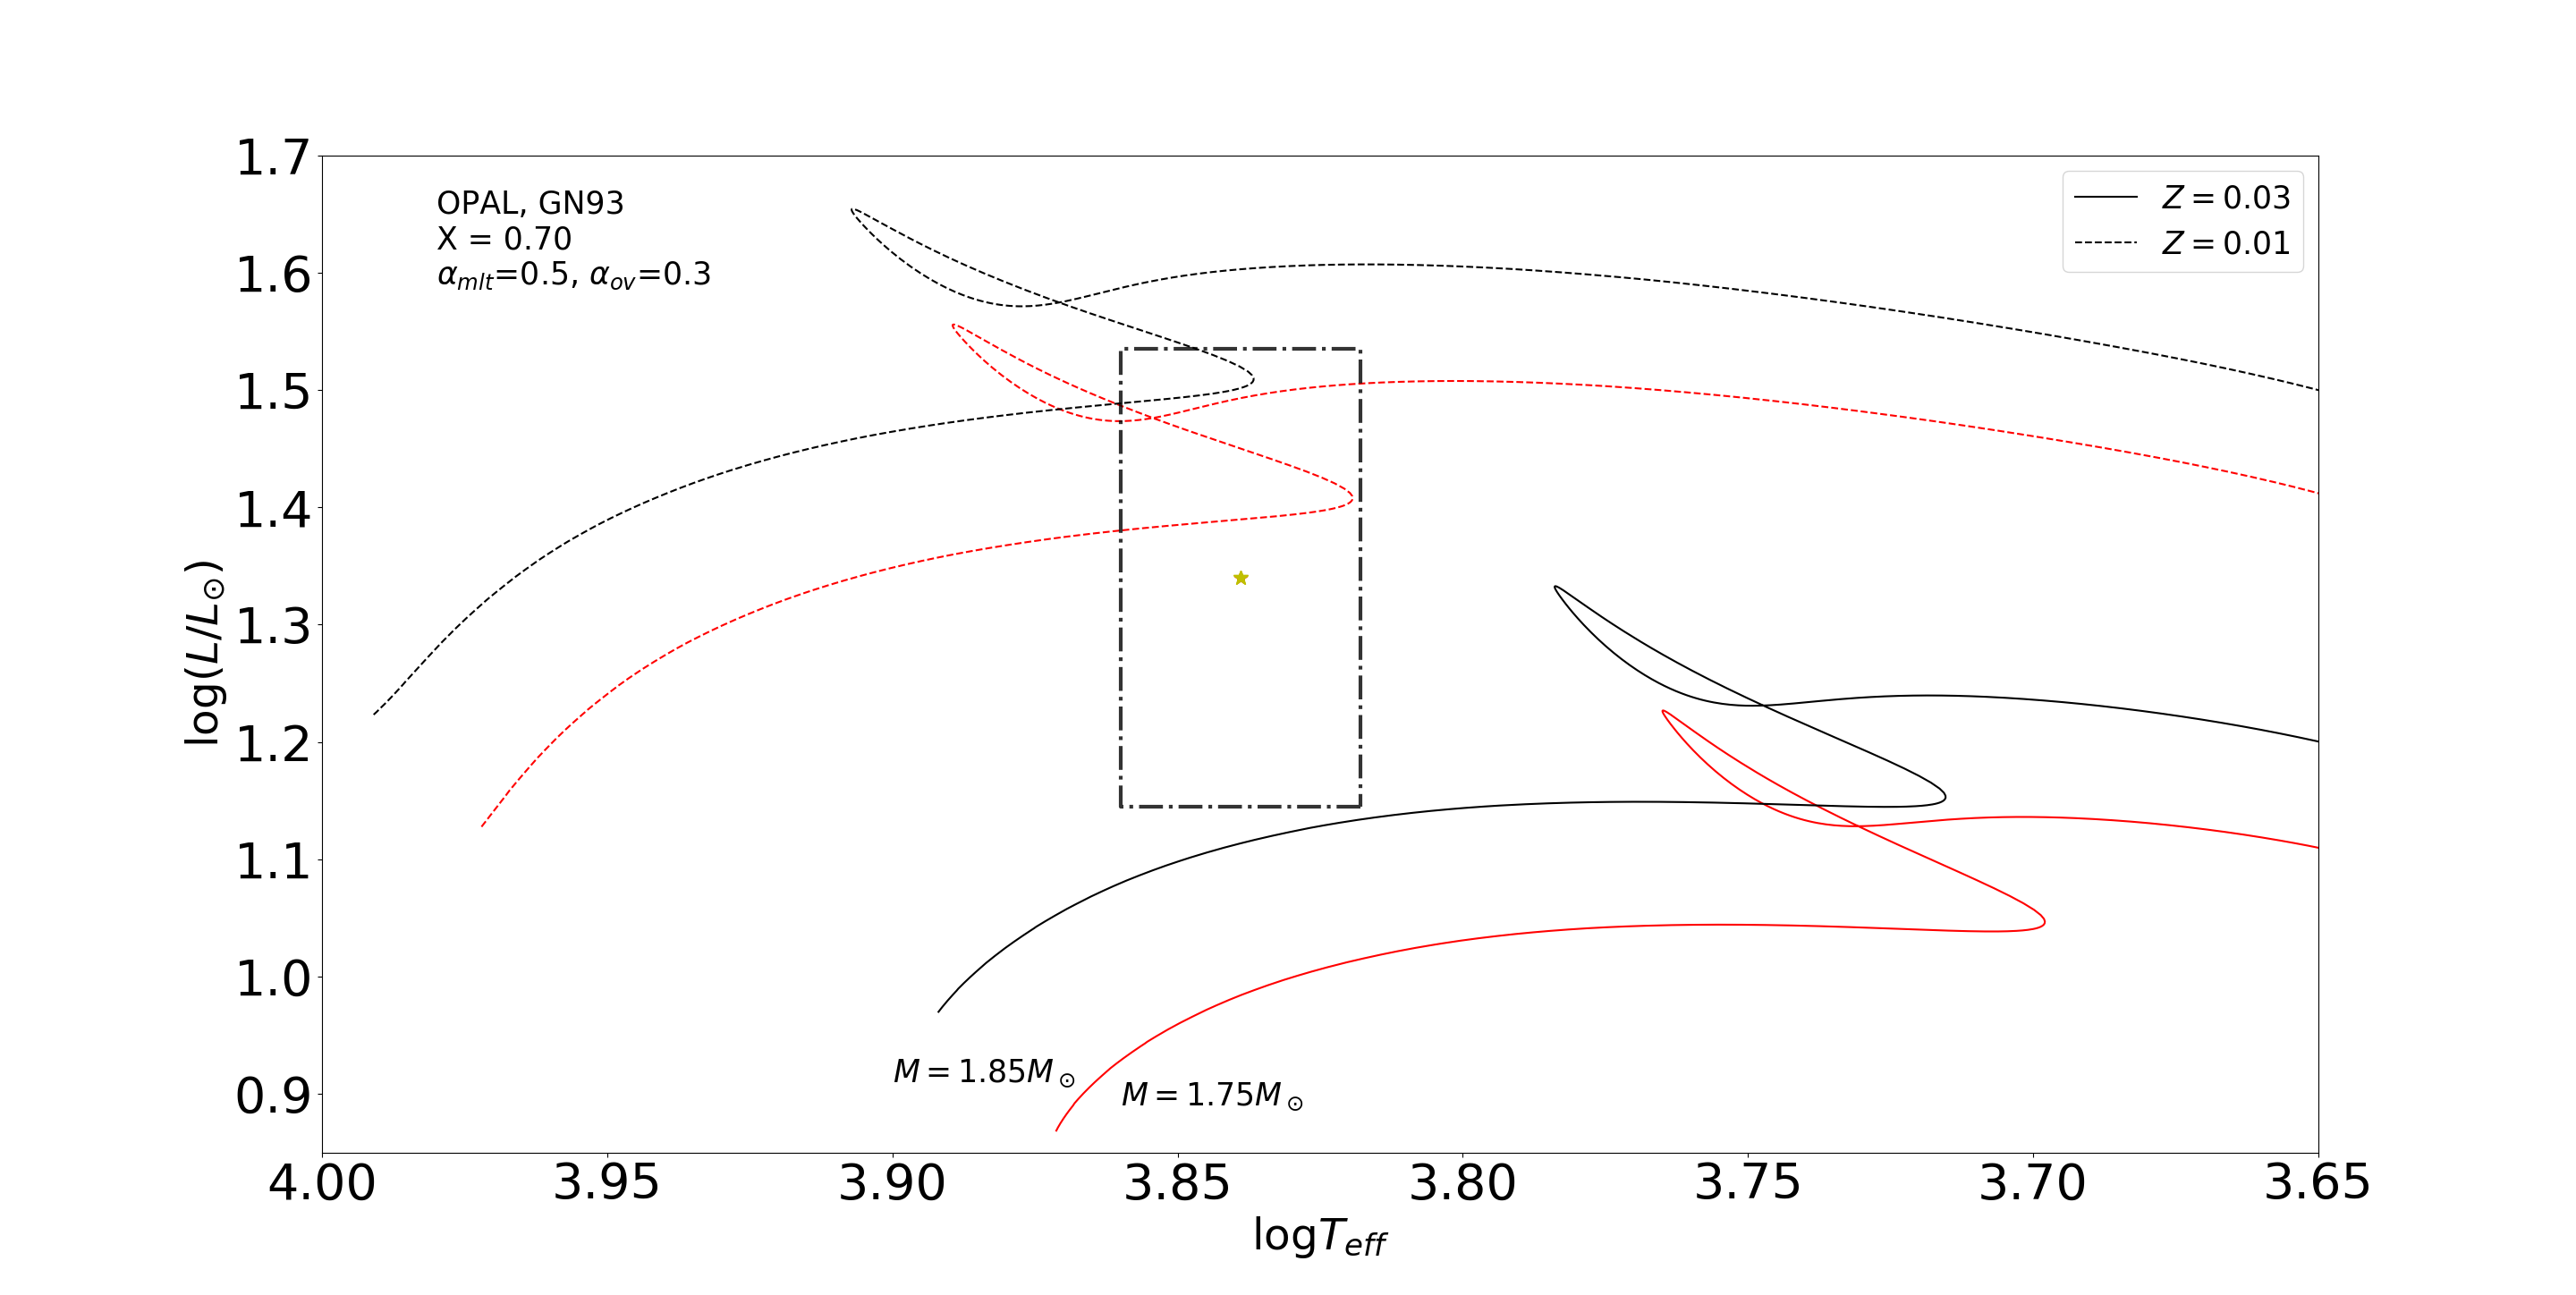
\includegraphics[width=0.9\textwidth]{test_z_2.png}
	\caption{Stellar evolution tracks for two different masses with two different metal abundances. Each track has $X=0.70$, $\alpha_{mlt}=0.5$ and $\alpha_{ov}=0.3$. The red lines indicates tracks with masses of $M=1.75M_\odot$, and black lines indicate $M=1.85M_\odot$. The full lines have $Z = 0.03$ and dashed lines $Z = 0.01$. The black dashed box shows the three sigma uncertainties on \l and \teff (from \citet{lenz2010delta}). }
	\label{diffz}
\end{figure}

Numerical results for the initial hydrogen abundances can be seen on \figref{diffx}. The line and color convention corresponds to that of \figref{diffz}, with the difference being the line type indicating the values of $X$ instead. Here it is also clear that the initial hydrogen abundance affects the luminosity (however less than the $Z$). Higher hydrogen abundances causes a smaller helium abundance (when $Z$ is held constant) HVORFOR ER LUM STØRRE?. 

\begin{figure}[htbp]
	\centering
	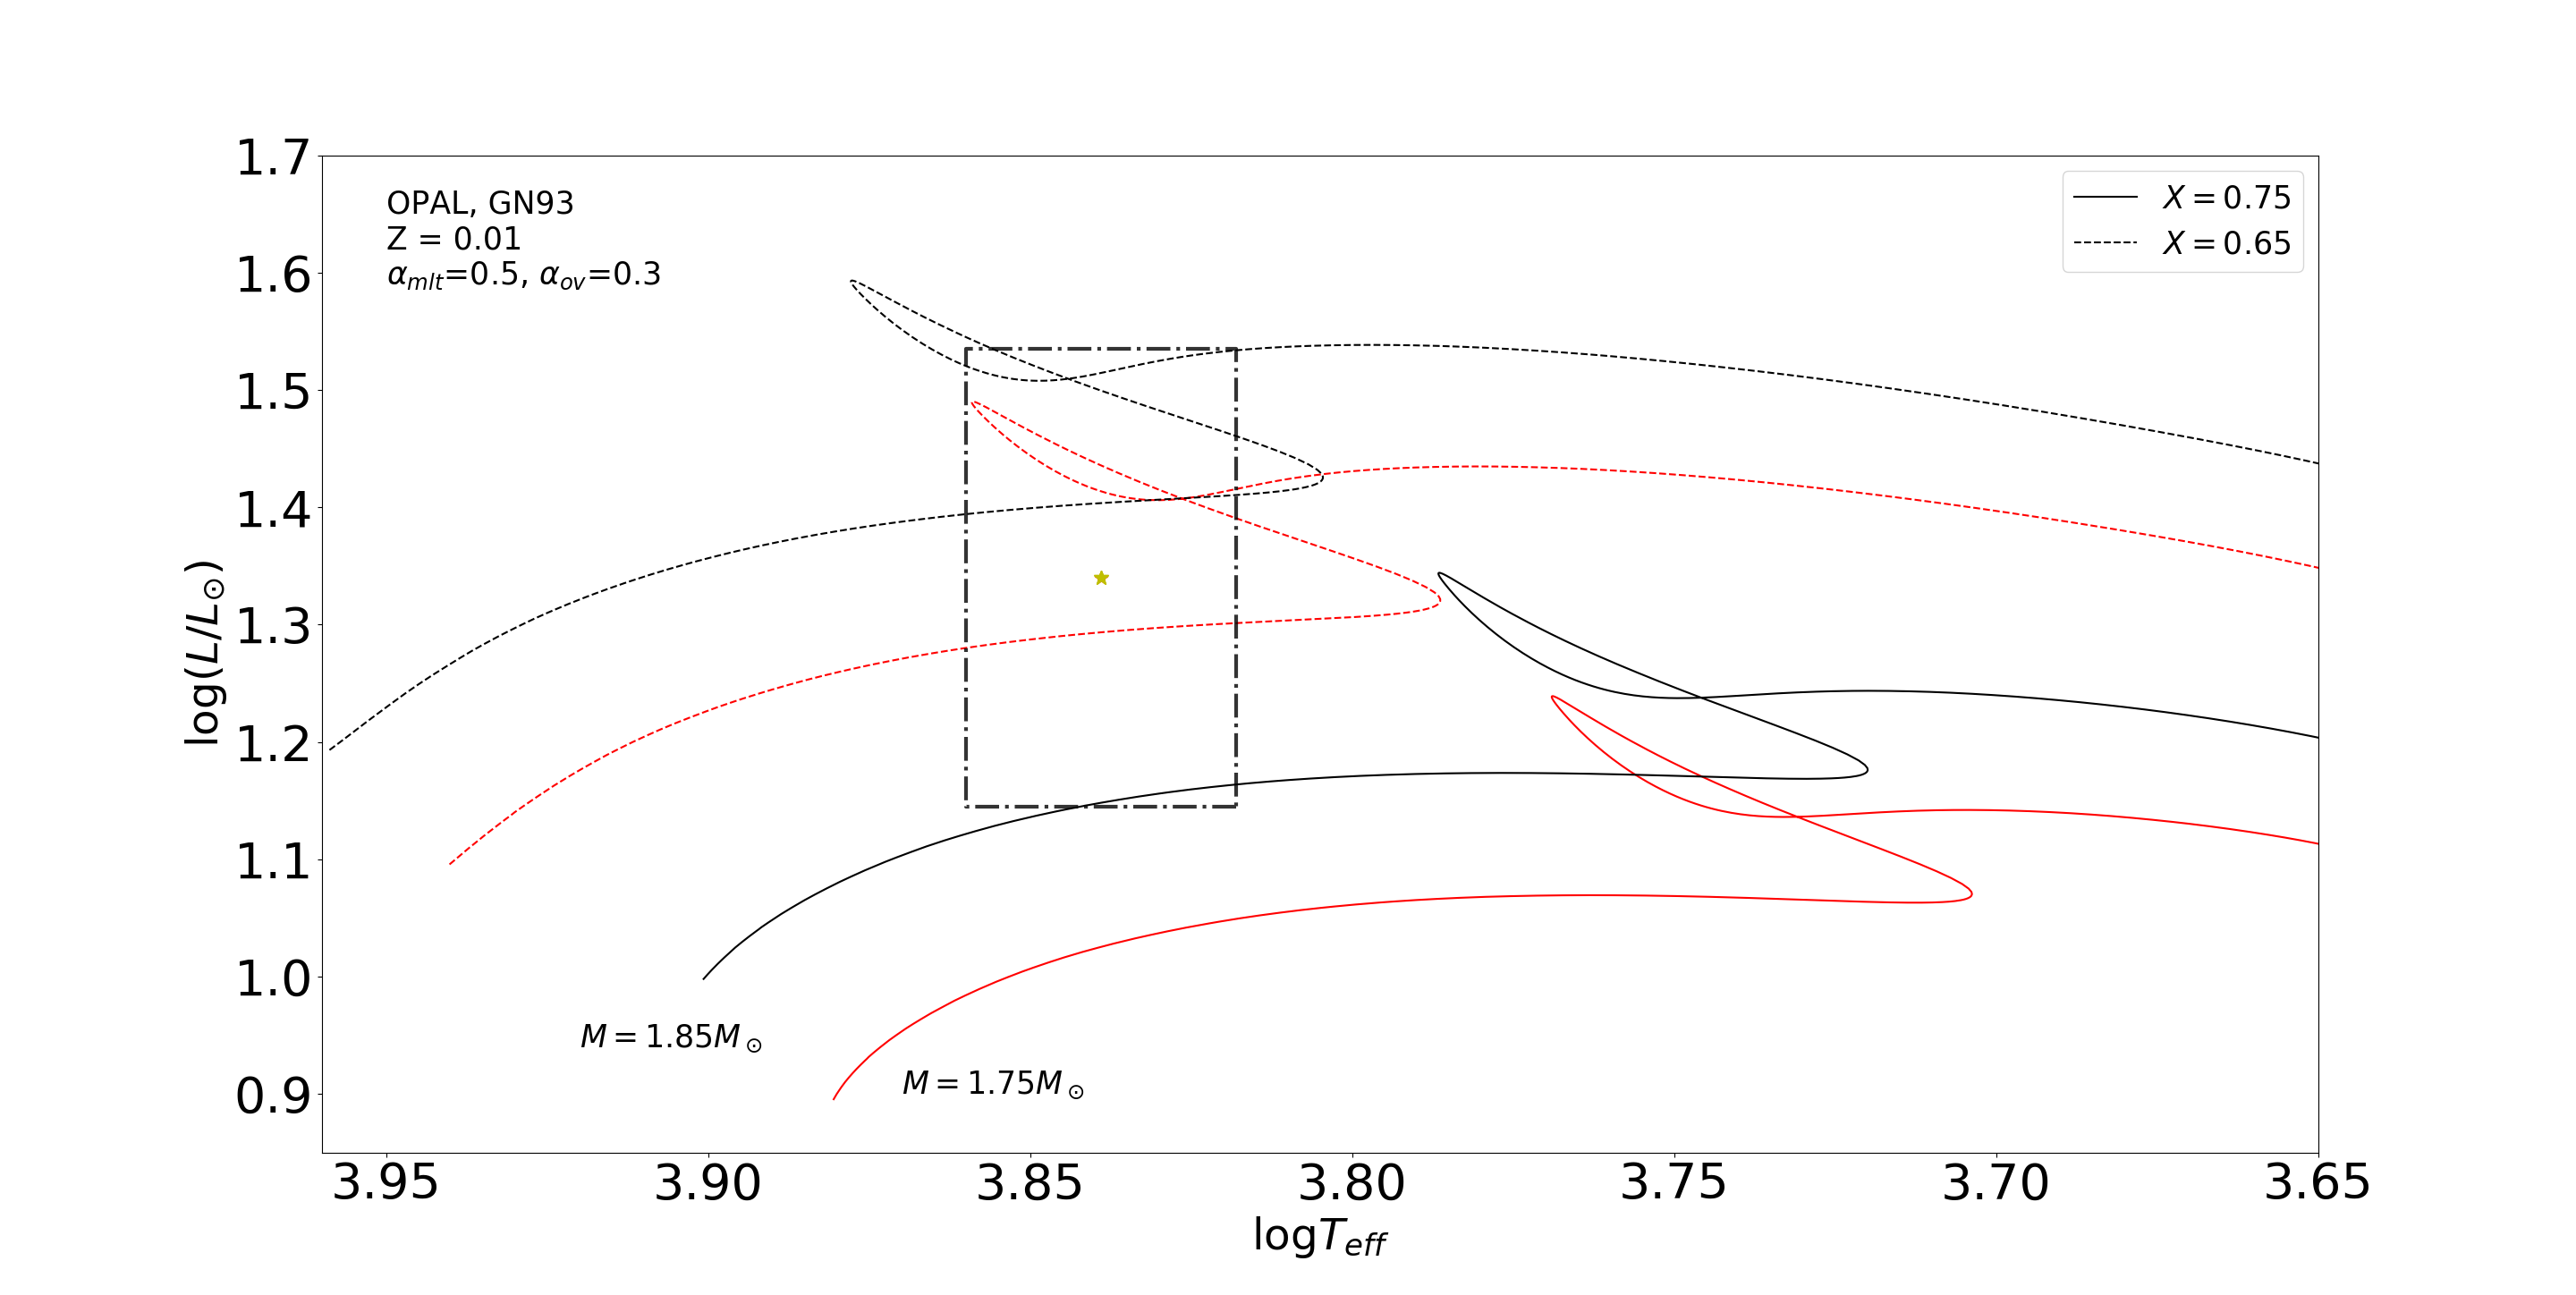
\includegraphics[width=0.9\textwidth]{test_x.png}
	\caption{Stellar evolution tracks for two different masses with two different metal abundances. Each track has $Z=0.01$, $\alpha_{mlt}=0.5$ and $\alpha_{ov}=0.3$. The red lines indicates tracks with masses of $M=1.75M_\odot$, and black lines indicate $M=1.85M_\odot$. The full lines have $X = 0.65$ and dashed lines $X = 0.75$. The black dashed box indicates the three sigma uncertainties on \l and \teff (from \citet{lenz2010delta}).}
	\label{diffx}
\end{figure}

 $\alpha_{mlt}$ and $\alpha_{ov}$ are parameters that are not easily chosen, since they are purely empirical and depend strongly on the prescription used in the modeling (see \secref{sec:conv_prescriptions}. For the $\alpha_{mlt}$ the standard value in \texttt{MESA} is around 1.8. The Warsaw-New Jersey stellar evolution code used to calculate models for 44 Tau by \citep{lenz2010delta} has the same mixing-length prescription as \texttt{MESA}. Their results showed that models with mixing length of $\alpha_{mlt} > 0.2$ gave the best fits, confirming the assumption that smaller mixing lengths than the sun is needed in order to model these stars. However, \texttt{MESA} is not computationally capable of handling a mixing length below 0.2 which is not surprising as it would mean that energy transport by convection in the outer layers is almost non existing. This also underlines the fact that convection is treated differently in each stellar evolution code, and parameters such as $\alpha_{mlt}$ needs to be carefully examined in the grid. It can also be argued that since $\delta$ Sct stars have a much smaller convection layer than that of the Sun, the convection will not be as efficient.  \citet{trampedach2011mass} calculated a range of mixing lengths through a grid simulation of solar type structures. One of the results can be seen on \figref{tramp}. 

\begin{figure}[htbp]
	\centering
	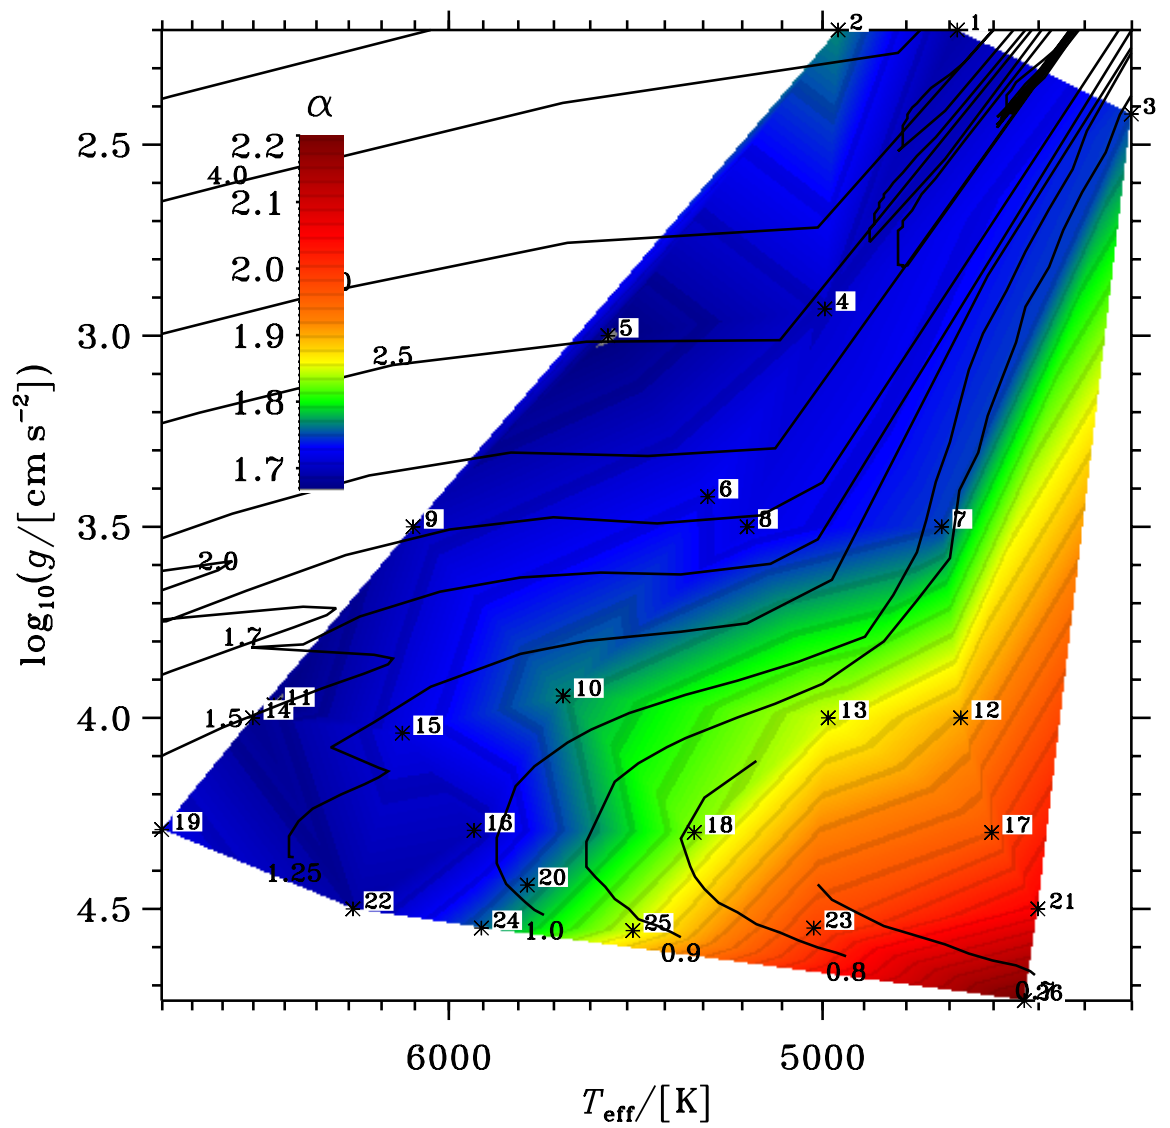
\includegraphics[width=0.8\textwidth]{tramper.png}
	\caption{Mass mixing lengths in units of pressure scale height $H_p$ in the \teff - $\log g$ plane. \citep{trampedach2011mass}.}
	\label{tramp}
\end{figure}

The mixing length is predicted to be smaller for higher values of \teff, as expected. Both 44 Tau and HD 187547 are out of range in \teff space, since the mixing length range here is calculated based on solar-like structures. However, the trend in mixing length is still applicable to intermediate mass stars. As an initial grid we therefore choose values of $\alpha_{mlt}$ between 0.2 and 0.8. Analogous to the mixing length, the convective overshoot near the core is described with the convective core overshoot parameter $\alpha_{ov}$. As it is typically in the order of 0.1-0.2 \citep{kippenhahn1990stellar}, we here choose values between 0.1-0.3.  

Some models in the grid were not possible to compute with the current equations in MESA. For 1.5\msun it was not possible to compute models with a metallicity higher than 0.02, it the initial He abundance is low. For 1.80\msun three tracks were excluded as they could not be computed either. The initial grid used here can be seen in \tabref{grid}.
\begin{table}[htbp]
  \centering
  \caption{Values and step sizes for all parameters in the grid calculated in this work. }
  \label{grid}
  \begin{tabular}{|l|ll|}\toprule
    & values    & stepsize \\ \midrule
    X                         & 0.65-0.75 & 0.05     \\
    Z                         & 0.01-0.03 & 0.01     \\
    Mass/\msun                & 1.5-2.2   & 0.05     \\
    $\alpha_{mlt}$            & 0.2-0.8   & 0.3      \\
    $\alpha_{ov}$             & 0.1-0.3   & 0.1      \\ \bottomrule
    \end{tabular}
\end{table}

Some of these combinations did however not converge properly, and could therefore not be included in the grid. These models are:
\begin{itemize}
	\item $M=1.50M_\odot$: combinations with $X=0.75$ and $Z=0.02$ or $Z=0.03$
	\item $M=1.55M_\odot$: combinations with $X=0.75$ and $Z=0.03$
	\item $M=1.95M_\odot$: combinations with $X=0.75$ and $Z=0.03$
	\item $M=1.80M_\odot$: combinations with $X=0.75$ and $Z=0.02$ and $\alpha_{mlt} = 0.2$
	\item $M=1.90M_\odot$: combinations with $X=0.75$ and $Z=0.02$ and $\alpha_{mlt} = 0.8$ 
\end{itemize}

It is unclear why these exact combinations have numerical issues, since it would require an investigation beyond the scope of this work. However, they all have in common that the initial hydrogen abundance is very high at $X=0.75$. This might explain most of the issues since this value is in fact higher than the initial value of the interstellar medium it was born in, which can practically never be true. However, the reason for still including them is that models might still reproduce these high values due to the numerical calculations. So if a model has this value it can be interpreted as an example of the imperfect theory behind the codes.  

\section{Resolution and varcontrol}
\label{sec:res}

As mentioned previously in \secref{sec:mesa}, they way MESA works is to fulfill calculations in time steps that are non-equidistant. As a result of this, models on a track can be far apart if the evolution is fast. This means that models on the main-sequence are well resolved, while the models on fast stages (particularly post-ms contraction phase) are fare apart in terms of structure. Since every model calculated in MESA yields one model in GYRE, this also results in the frequencies being very different from one model to another, which should be considered when calculating the \chis (see \secref{sec:chis}). An example can be seen on \figref{resstage} where, the radial fundamental mode is plotted as a function of timestep. The lower panel of \figref{resstage} is the same models corresponding to middle panel but where the radial fundamental mode frequency difference between models, $f_1(i+1) - f_1(i)$, is plotted as a function of time. This shows that the resolution in the frequency space is as high as ~0.18 cyc/day for this track (some tracks go up to ~0.2). The highest point is, however, in the very beginning of the main sequence, and not on the post-main sequence contraction phase, where it is favorable to have a high resolution.     

\begin{figure}[htbp]
    \centering
    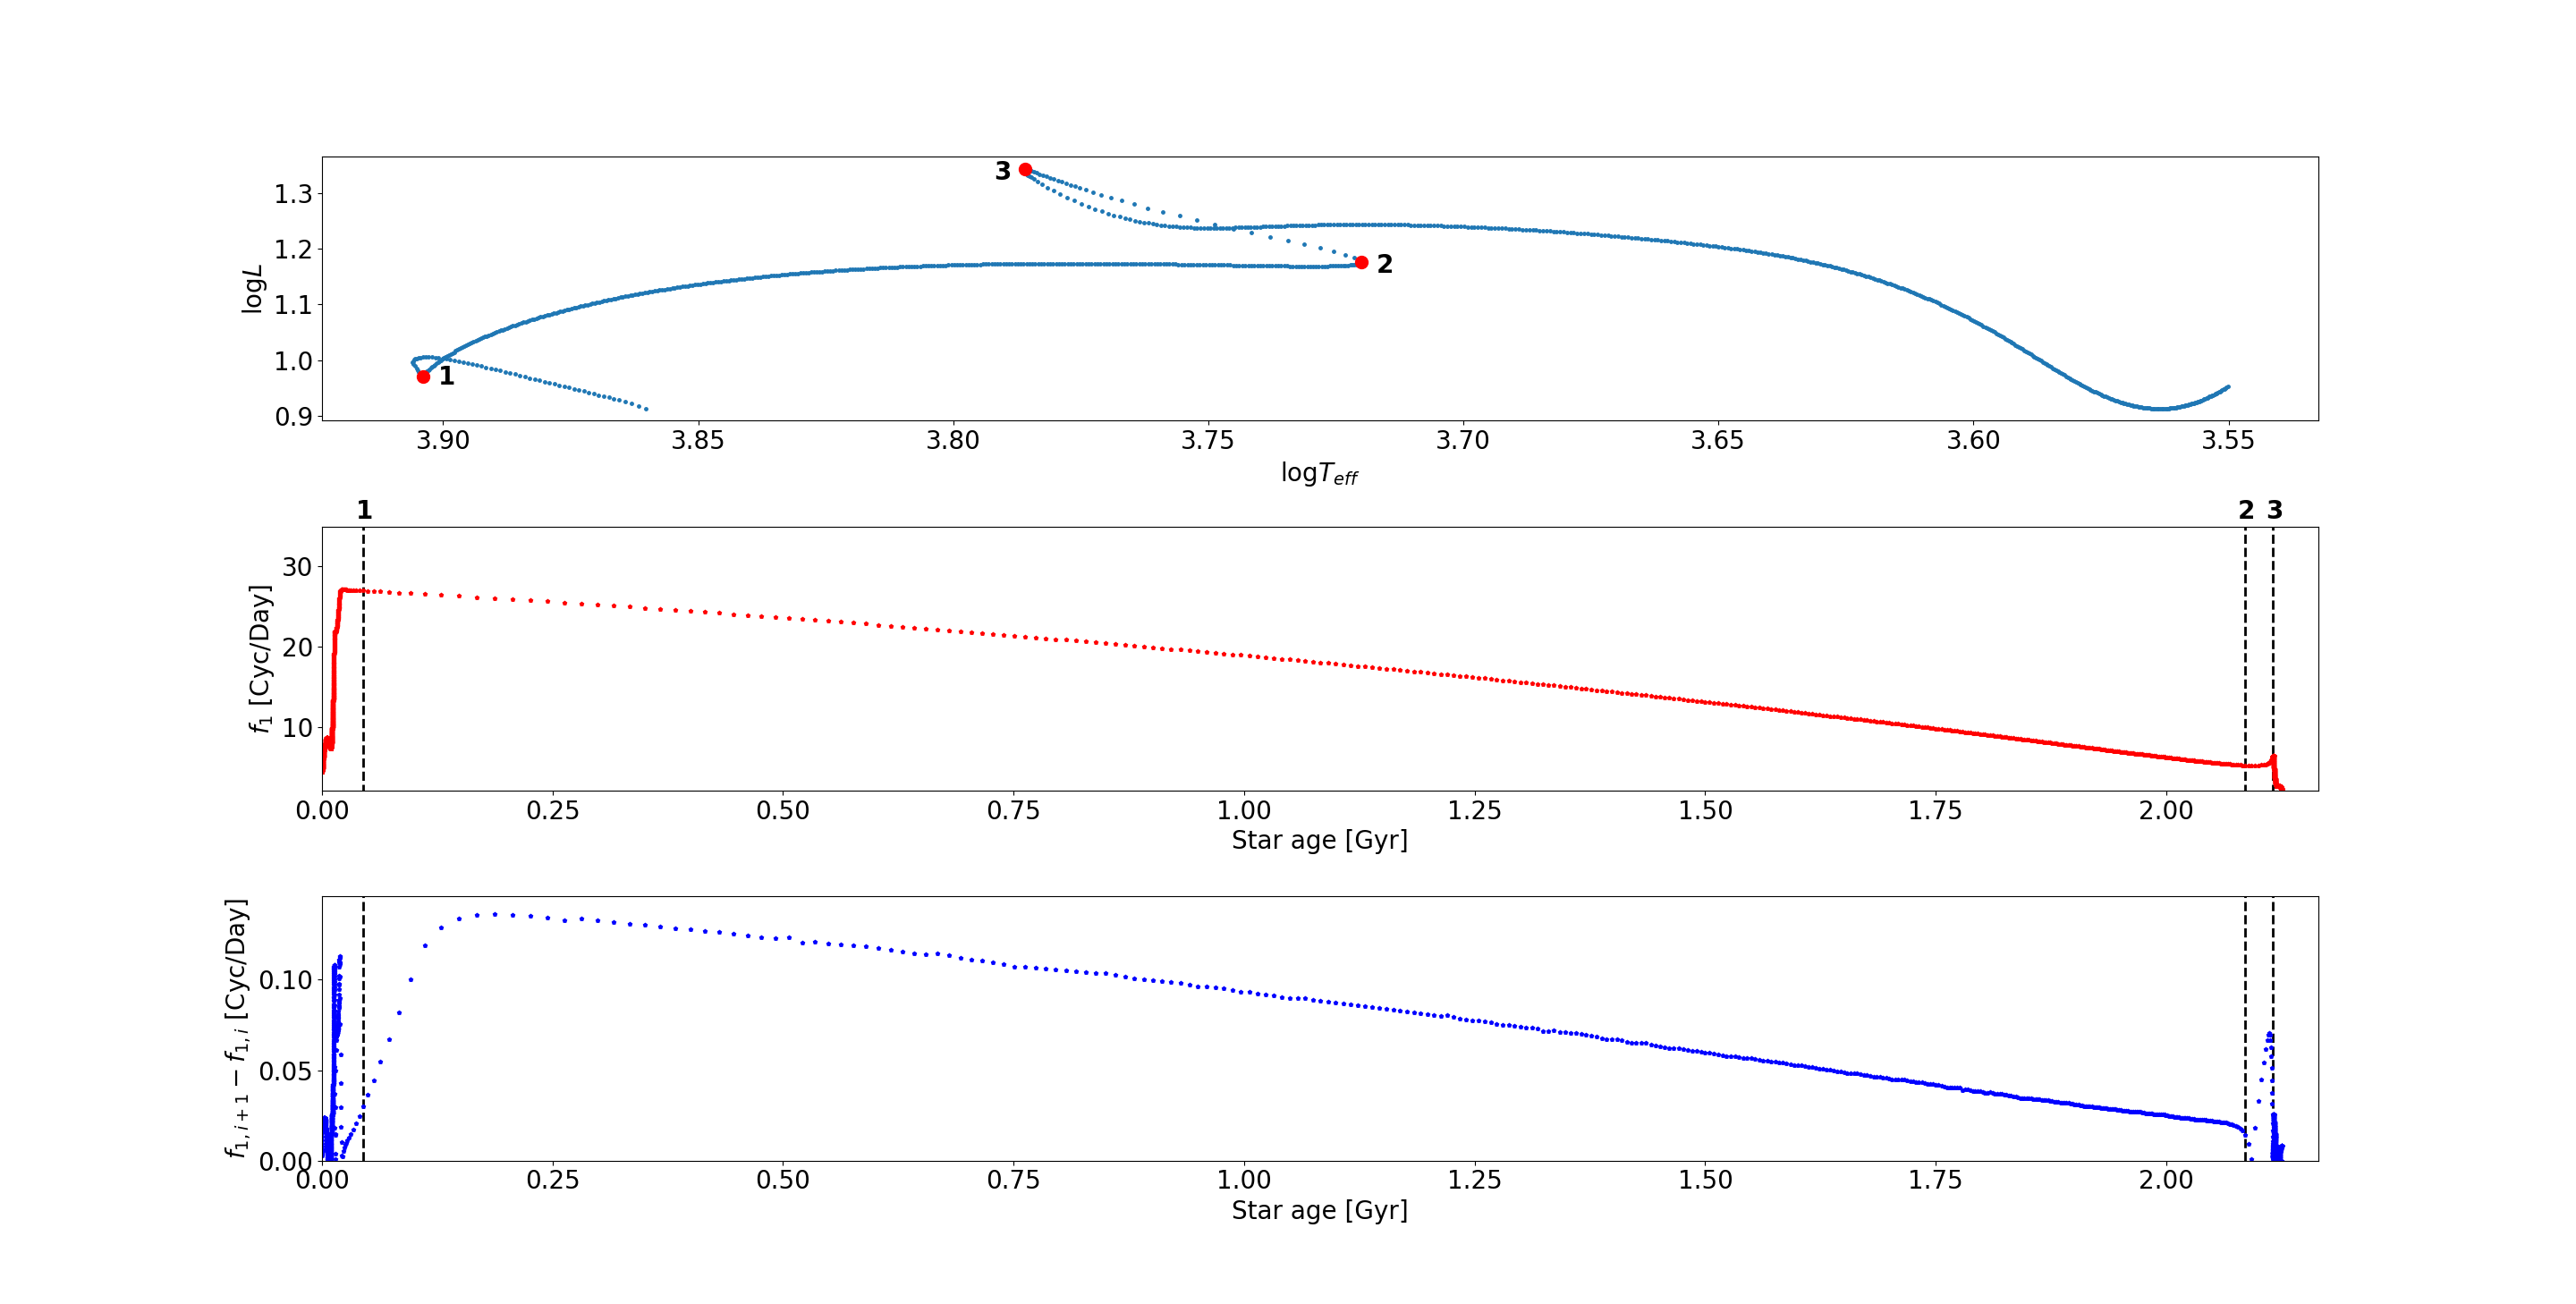
\includegraphics[width=1\textwidth]{resolution_stages.png}
    \caption{Resolution at different stages of an evolution of a track with M=1.85\msun, X=0.75, Z=0.02, $\alpha_{mlt} = 0.5$, $\alpha_{ov} = 0.3$. The begininng of the main sequence is marked with a bold "1", continuing until "2" where the post-main sequence contraction phase starts. At "3" all hydrogen has been exhausted in the core, and the star is in the post-main sequence expansion phase. Middle panel: Here the fundamental frequency is plotted as a function of time. The dashed lines indicate the stages corresponding to those in the middle panel. Lower panel: Shows the absolute difference in fundamental frequency between two subsequent models.}
    \label{resstage}
\end{figure}

Since 44 Tau has earlier been identified to be in the post-ms contraction phase (and since we cannot exclude that possibility for Superstar either) the resolution of the models in MESA needs to be adjusted to allow for a higher chance of finding a good fit. It is possible to simply force smaller timesteps, but this is not ideal since it would not only increase the computation time on the fast evolutionary stages, but the entire track. Since a better resolution is not really needed on the ms, it is therefore better consider an alternative parameter that does not waste computation in areas where it is not needed. 

There are more than one way of doing so. It is possible to set a limit for magnitude of max change in temperature and photosphere with the \texttt{delta\_lgTeff\_limit}, or alter the minimum and maximum number of grid points in a model with \texttt{mesh\_delta\_coeff} (a higher values decreases number). These parameters need to increase the resolution in the right area, but also within a resonable amount of computation time. The parameter found to be most efficient in this project is the \texttt{varcontrol\_target} parameter. This parameter is assigned a value describing the relative variation in the structure from one model to the next. The timestep then adjust accordingly, depending if the variation is smaller or larger than the value. Increasing the resolution through this value does also increase the computation time, however, reasonably. An example of this can be seen on \figref{varcontrol} where the same track is plotted with different values of \texttt{varcontrol\_target}. It is here found that a value of 5e-5 is sufficient in making the resolution satisfactory for this work. 

\begin{figure}[htbp]
    \centering
    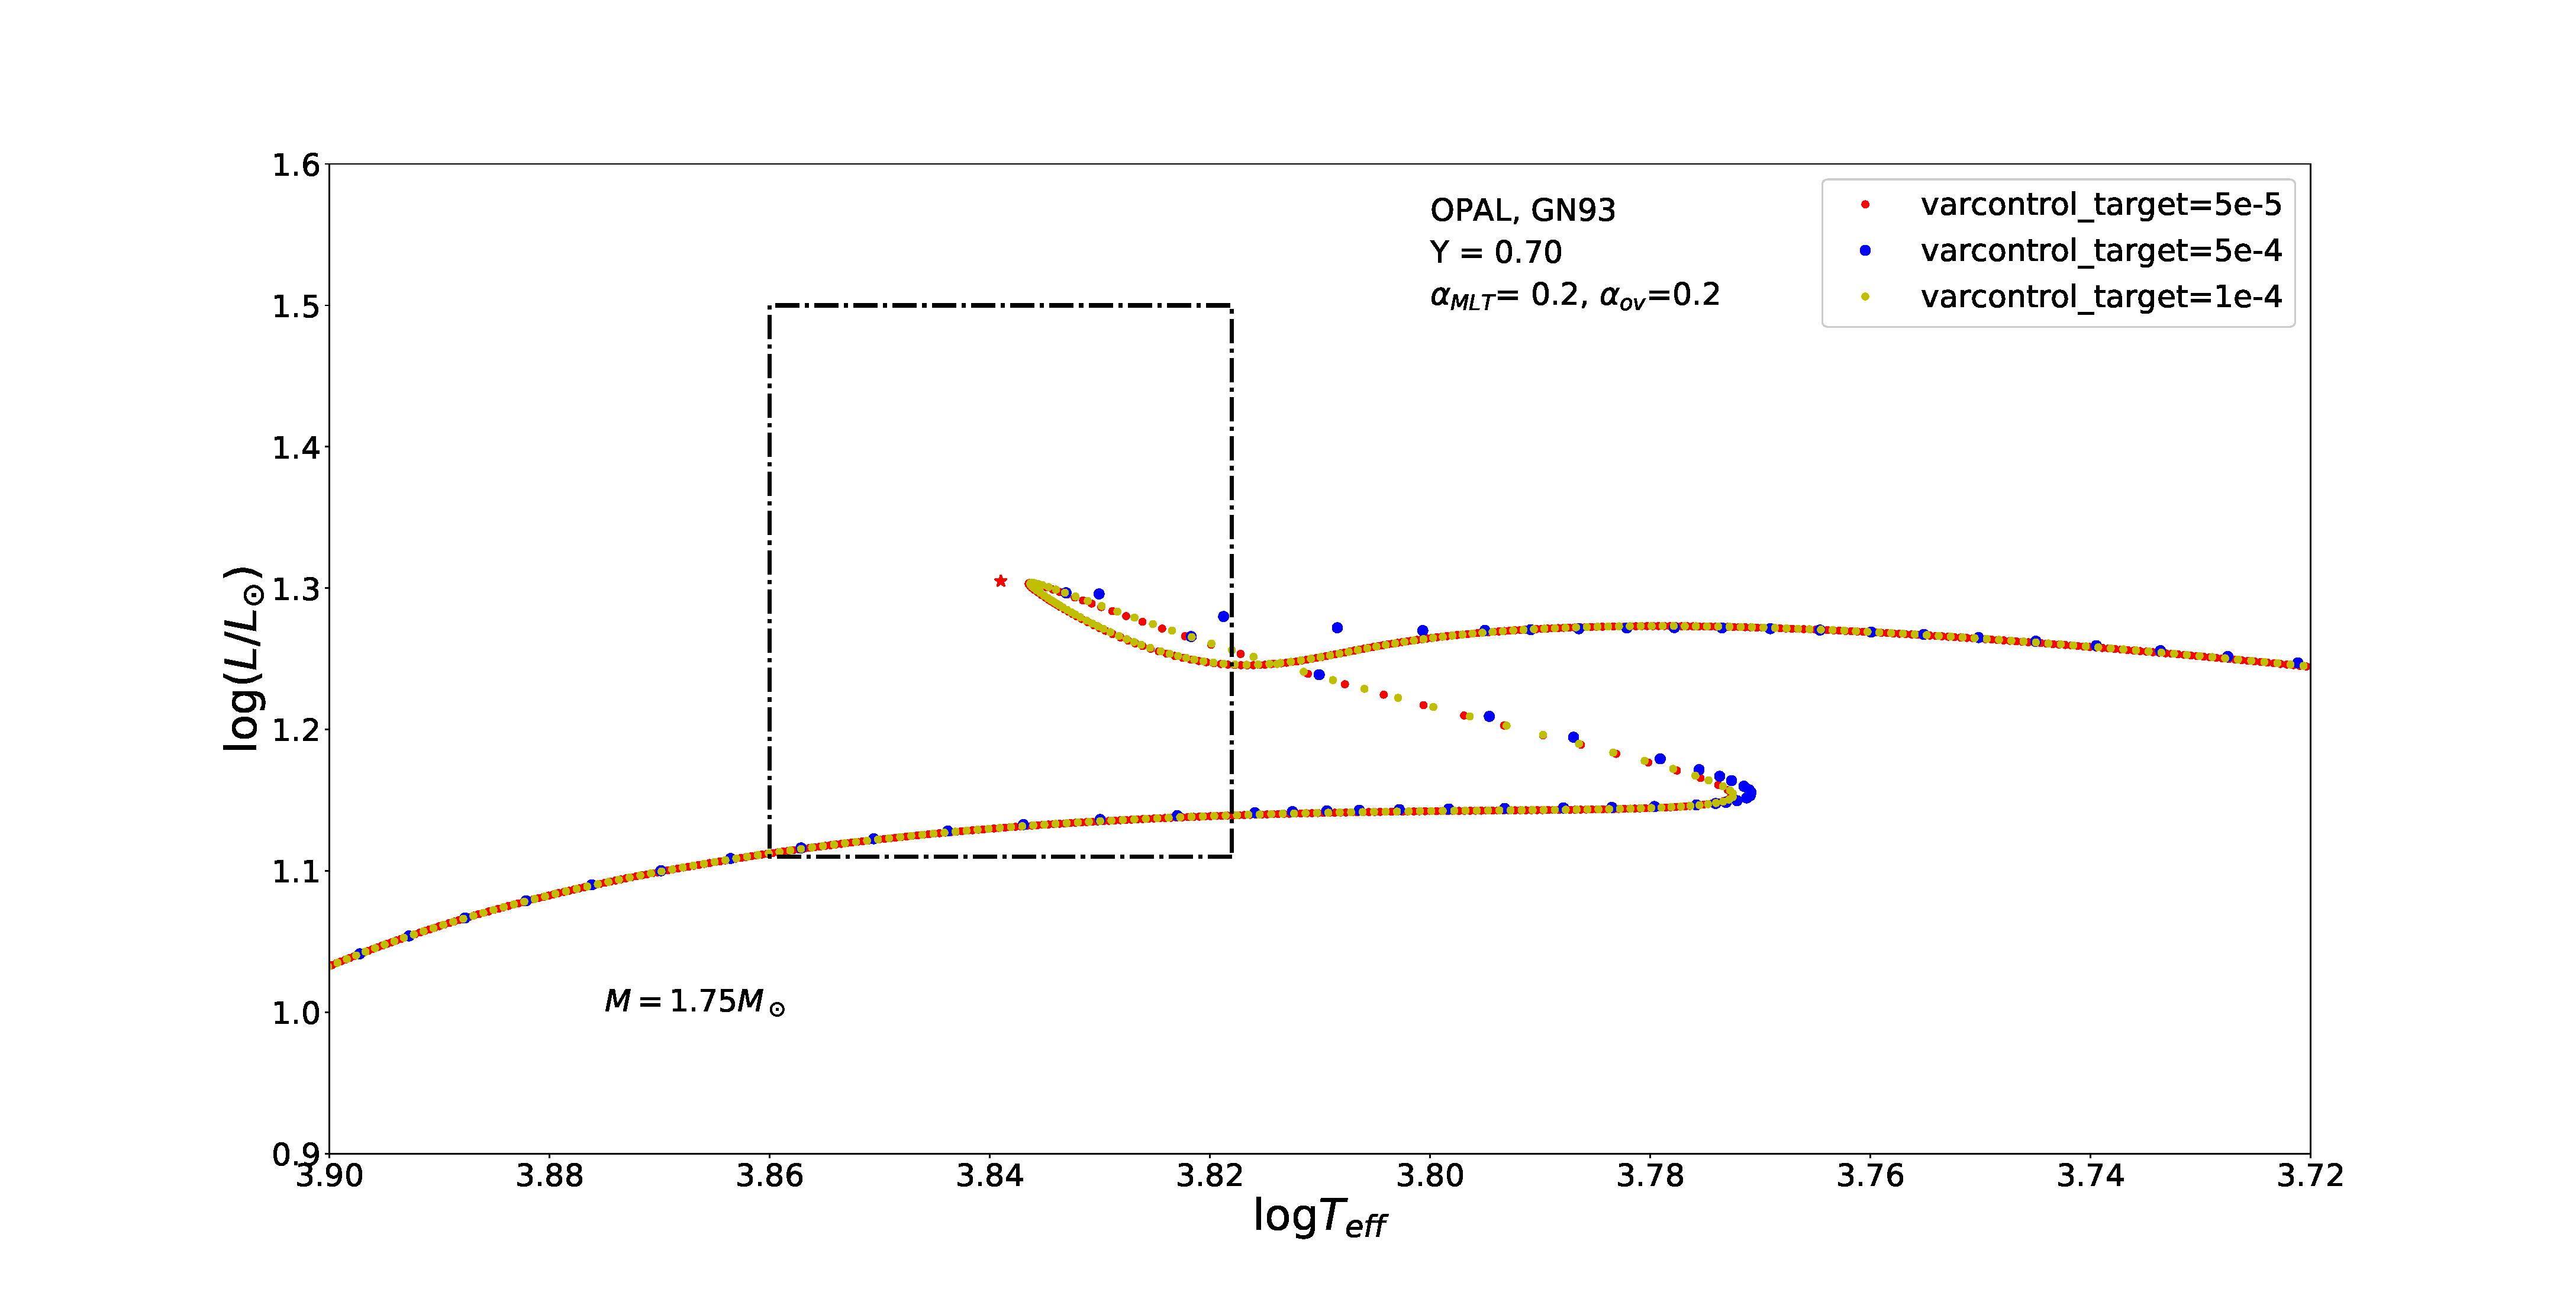
\includegraphics[width=1\textwidth]{varcontrol_res.eps}
    \caption{Evolution of three tracks with same initial parameters, but different values of \texttt{varcontrol\_target} where 1d-4 is default in \texttt{MESA}. It can be seen that the resolution drops significantly for the value 5d-4. Therefore, a slightly smaller value of 5d-5 is chosen for this work.}
    \label{varcontrol}
\end{figure}


Some tracks are still better resolved than others. A general tendency from the computed tracks are that models with overshoot below 0.2 are not resolved nearly as well as models with high overshoot of 0.3, which can also be seen on \figref{ovresol}. Particularly the Henyey hook cannot be reproduced very well for overshoot of 0.1. The details as to why this occurs is beyond the scope of this work, however it is very important to take into consideration when evaluating results as tracks with low overshoot will automatically have fewer models and therefore limited chances of fitting well to observations. 

\begin{figure}[htbp]
    \centering
    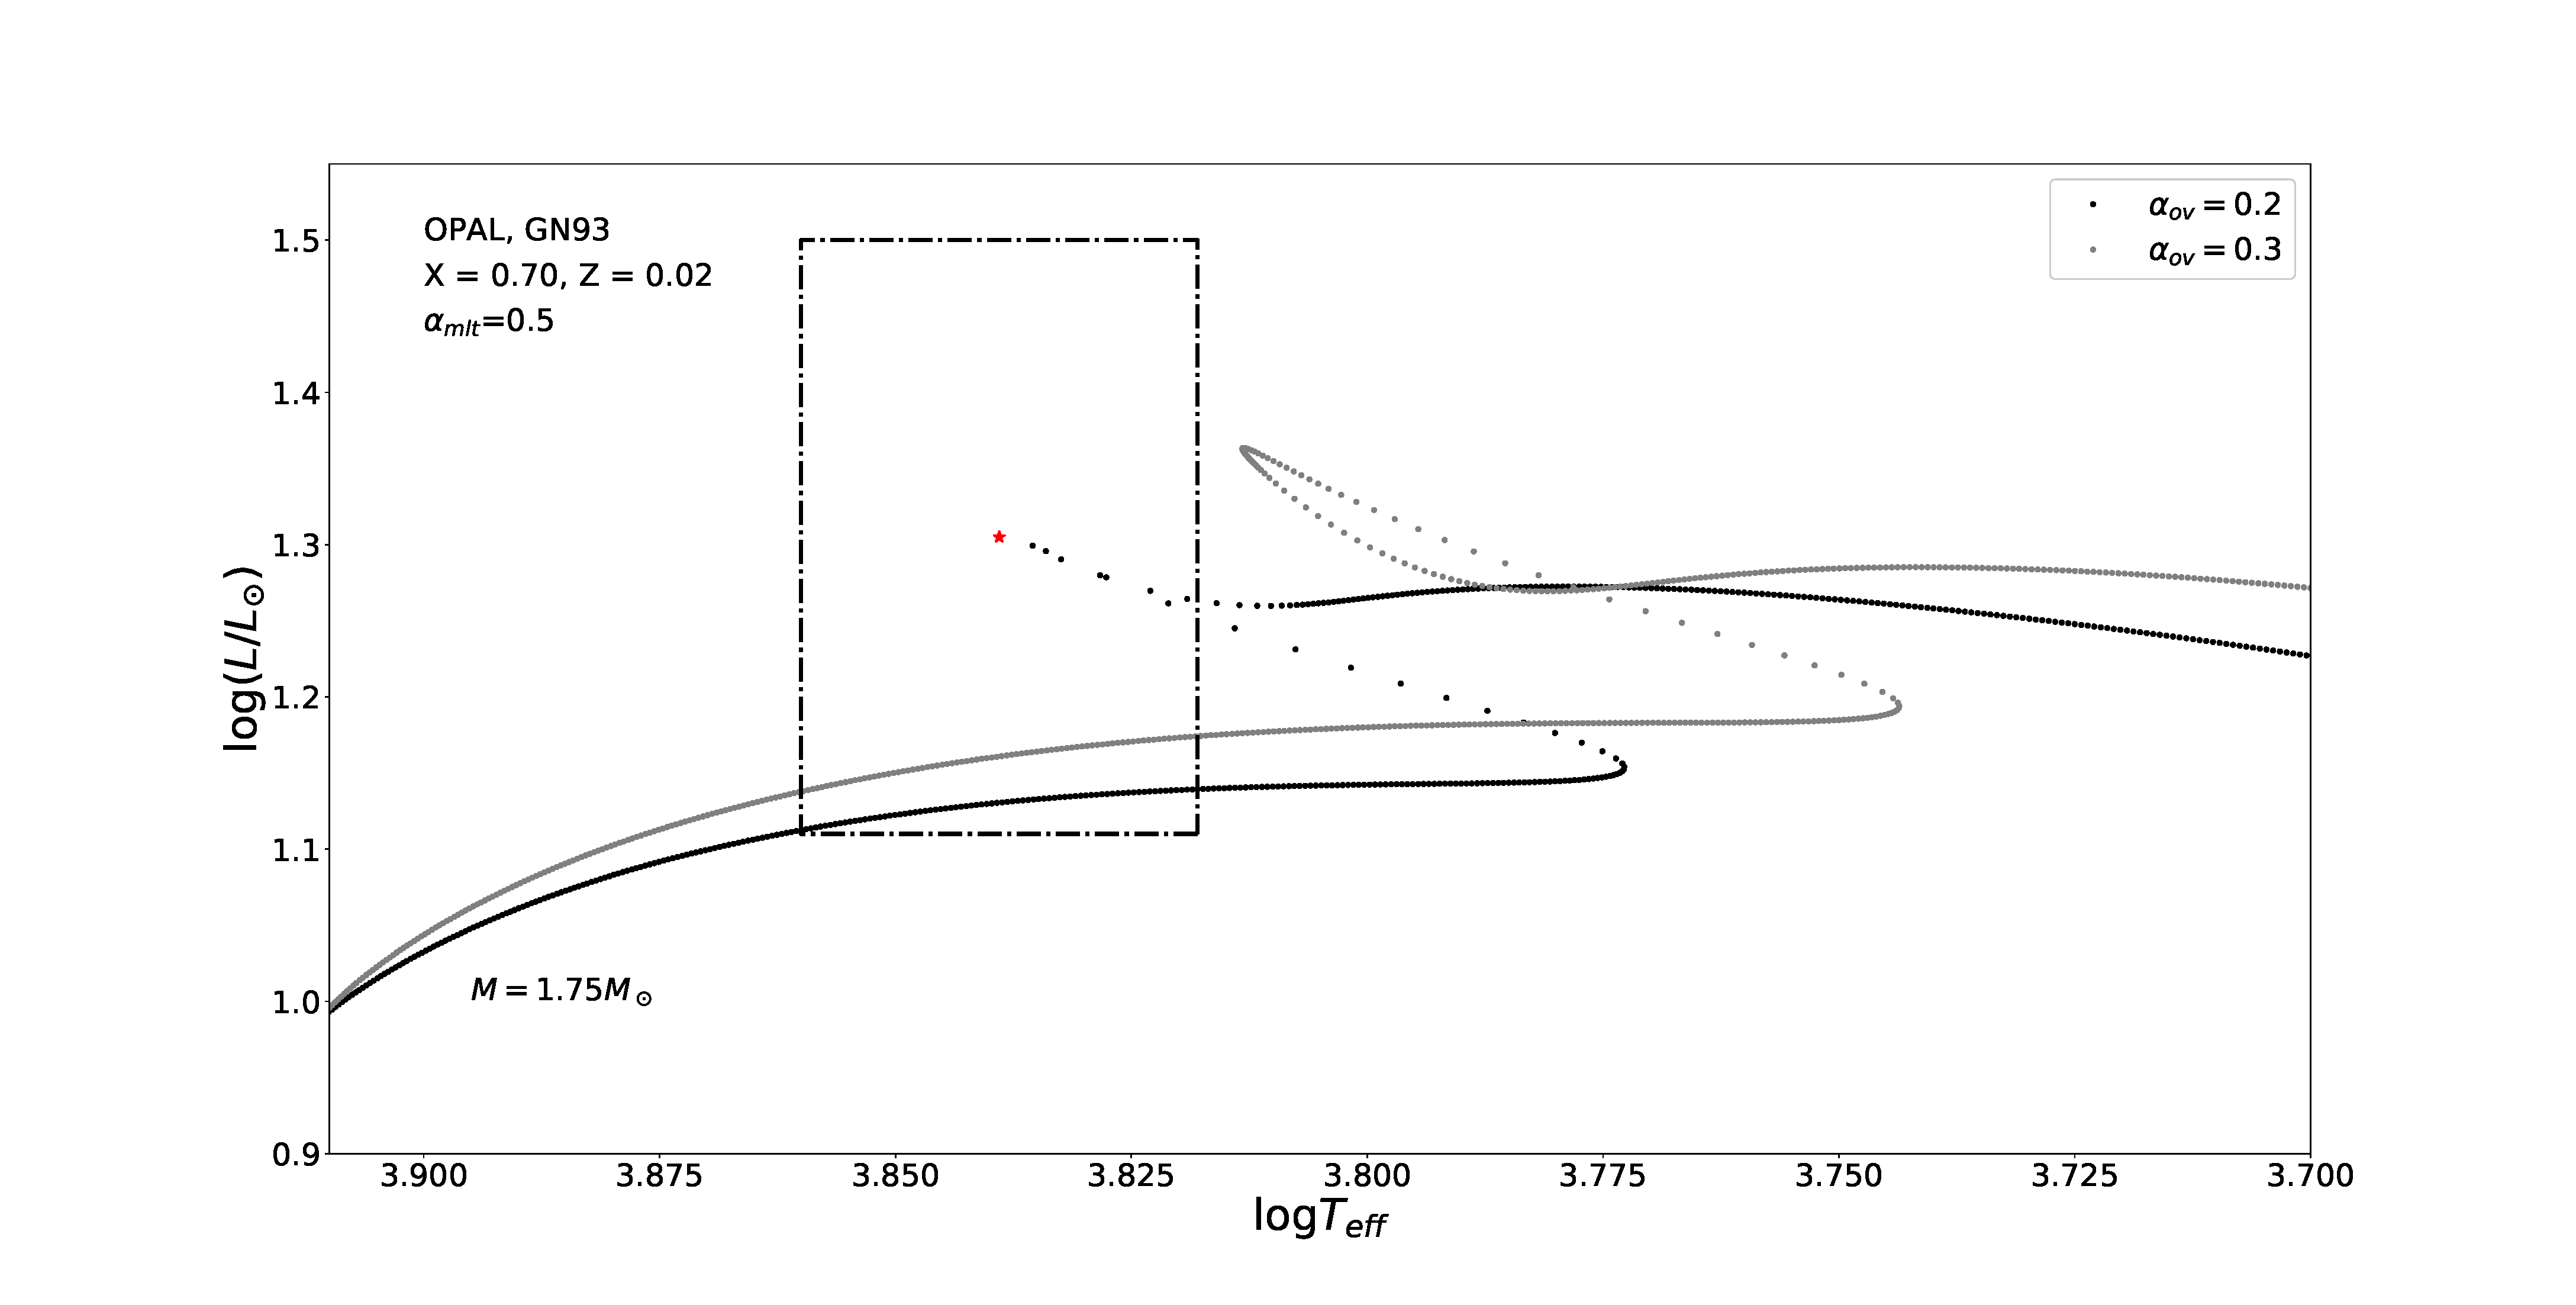
\includegraphics[width=1\textwidth]{resolution_overshoot.eps}
    \caption{Two models of the same track, but with different overshoot.}
    \label{ovresol}
  \end{figure}


\section{chi2 testing}
\label{sec:chis}

\subsection{Finding the best model}
\label{bestmodel}


In order to find out how well/fitted a model is, a comparison with stellar parameters is needed. By just comparing models to luminosity, effective temperature and surface gravity, it is difficult to find an estimate on the evolutionary stage as the best model on one track might be on the main sequence, whereas the best model on a different track is on the post-main sequence. Therefore, frequencies are need as additional observational parameters for comparison (as they, as discussed in \secref{chap:asteroseismology}, change with evolution). There is more than one way of doing the comparisons, but in this work a \chis test is used. \chis yields a value for each models, allowing us to find models with lowest \chis values. The Pearson's goodness of fit test is commonly written as 

\begin{align}
\label{standard_chi}
\chi^2_j = \sum^I_{i=1}\left(\frac{v^{theo}_{i,j}-v^{obs}_i}{\sigma_i}\right)^2,
\end{align}

\noindent where $\nu^i_{obs}$ is the observed parameter for model i, $\nu^i_{theo}$ is the corresponding theoretical parameter and $\sigma^i$ is the uncertainty for the parameter. It provides a number that somewhat describes how close the fitting parameters are tp the corresponding observed parameters. However, there is more than one way of doing a \chis test, as its implementation depends on the work, and particularly the goal that is desired. There are a few assumption that needs to be taken into consideration before implementing a \chis test. Most importantly, statistically speaking, a \chis test does not provide any information on how well individual parameters fit, or how likely a model is to be good. As the goal of this project is to find the most likely evolutionary stage, the \chis values can simply be used as a way of \textit{comparing} between the different models. So models with the lowest \chis are the models with parameters closest to the observed parameters. These thereby provide an age span and a likely evolutionary stage. 
If the \chis values are to be compared between the different models, then they need to be calculated under the same conditions. This means that calculations should be done with the same number of fitting parameters for all models (since they otherwise are not comparable). For instance, if one model have more fitted frequencies than another, the \chis with the model with more fitting parameters will have an extra link, causing it to naturally be larger than the \chis for the model with fewer fitted frequencies, making their \chis incomparable. 

%GYRE produces an output file for the chosen MESA profiles. Since it computationally takes time to produce the output files, a constraint is needed in order to determine which profiles are within the range where we wish to produce a GYRE output file. This is done by defining a parameter space of size three sigma, based on observed parameters \teff, \lum, and \grav.

%In order to test how well the computed frequencies match observed frequencies a \chis prescription is applied to every profile. 
\subsection{44 Tau}
\label{sec:chi44}

\subsubsection{l=0 modes}

For 44 Tau, the frequencies of the fundamental mode and first overtone are well-determined. These frequencies act as a constraint for the l=0 mode models. Initially the l=0 modes are computed using GYRE for the entire grid described in \secref{sec:grid}. Here, we have an initial constraint from only the frequencies corresponding to the radial fundamental mode and first overtone and the global parameters. The \chis for this initial run then becomes

\begin{align}
\chi^2_j & = & \left(\frac{\nu^{\text{fund,obs}}-\nu_j^{\text{fund,theo}}}{\sigma_{\text{fund},j}}\right)^2 
 + \left(\frac{\nu^{\text{first,obs}}-\nu_j^{\text{first,theo}}}{\sigma_{\text{first},j}}\right)^2 
 +
\left(\frac{\text{T}_\text{eff}^{obs}-\text{T}_{\text{eff},j}^{\text{theo}}}{\sigma_{\text{T}_\text{eff},j}}\right)^2 \\
& & +
\left(\frac{\log \text{g}^\text{obs}-\log \text{g}^\text{theo}_j}{\sigma_{\log \text{g},j}}\right)^2 
 + \left(\frac{\log \text{L}^{\text{obs}}-\log \text{L}^\text{theo}_j}{\sigma_{\log \text{L},j}}\right)^2, 
 \label{eq:chis}
\end{align}

\noindent where $\chi^2_j$ is the \chis for the j'th model. For $\text{T}_{\text{eff}}$, $\log \text{g}$ and $\log \text{L}$ the $\sigma$ used is simply the uncertainties from observations. Notice here that even though the frequencies are calculated for the entire track, the \chis is not calculated for models on the pre-main sequence. 

For the frequencies the $\sigma$ is naturally very small (in the order of $10^{-6} \text{Cyc}/\text{day}$, since the uncertainty on observations depend only on the observation time. Long observation times of 44 Tau therefore results in very narrow peaks. It is very nice to know a parameter to this precision, but as shown in \eqref{eq:chis} a small uncertainty will results in high values of \chis. This is not a problem on its own, as the \chis only represent how well the model fits observation. If this value is extremely high it does not necessarily mean that the models are not good models for the star, but that a model precision is simply not comparable to frequency precision. In other words, no model will ever get close to fitting well. Also, by only dividing by the uncertainties the resolution of the track is not taken into consideration. As shown in \secref{sec:res} the resolution of the track is important as fewer models in one area decreases the possibility of having a good fit. This also means that a model frequency can change a lot between two time steps if the resolution is low, and this should be taken into account. In this work the following is prescription is therefore applied to the frequencies: 
\begin{equation}
\label{sigma}
    \chi^2  = \frac{1}{\alpha}\sum^I_{i=1}\frac{\left(v^{\text{obs}}_{i}-v^{\text{theo}}_{i,j}\right)^2}{(\sigma^{\text{obs}}_i)^2 f_i(\Delta\nu_{i,j})}
\end{equation}

\noindent where i in this case is the different frequencies (i.e I=2 for l=0 calculations where we only compare to fundamental frequency and first overtone),j is the j'th model, and $\alpha$ is a scaling parameter. $f_i(\Delta \nu_{i,j})$ is a function that artificially increases the sigmas on the frequencies

\begin{equation}
\label{function}
    f_i(\Delta \nu_{i,j}) = \frac{\nu_j - \nu_{j-1}}{\sigma_{\text{obs},i}},
\end{equation}
 
\noindent where the distance in frequency space is taken into consideration for the j'th model. Smaller distances in the frequency space between model means a higher $f_i(\Delta \nu_{i,j})$, hence, as smaller \chis. Runs both with and without the uncertainty pump will be made to test the difference in the main result. 

%Alternatively, the \chis for the frequencies can be calculated as \eqref{standard_chi}, but with an expanded $\sigma$ similar to that of a standard deviation

%\begin{equation}
%\label{m2}
   % \sigma_{i,j} = \frac{1}{I}\sqrt{\sum_{i=1}^I \left(\nu_{i,j}^{\text{theo}} - \nu_{i}^{\text{obs}}\right)^2}.
%\end{equation}

%There are both advantages and disadvantages for both methods. The first method does take the spacing into consideration, but it follows from this that the since the \chis are artificially enhanced, the scaling between the frequency \chis and rest of the parameters is off by the scaling factor $\alpha$. This can be found by finding the ratio $\frac{\chi_{freqs}}{\chi_{freqs}}$ for each model, j, and finding the mean. This method is slightly more complicated than the second method, however, the second method does not take the spacing in frequency between models into account, and the standard deviation is based only on two different frequencies. The order of magnitude of the \chis is different for the methods, but as mentioned earlier the numbers themselves are not representative of how well a model fits. 

As of yet only l=0 modes have been fitted. Calculating corresponding l=1 and l=2 modes for all models is time consuming, and therefore a selection criteria is needed. This is done by first finding the model with the lowest \chis is for each track. From all of these the best 5\% are found for both methods, respectively. These models and their initial parameters are shown in \tabref{bestchi_m1} and \tabref{bestchi_m2}. 

\begin{table}[htbp]
  \caption{hest}
  \label{bestchi_m1}
  \begin{tabular}{lllllllllll}
 Model & X & Z & Y & $M[M_\odot]$ & $\alpha_{mlt}$ & $\alpha_{ov}$ & $\log \text{T}_\text{eff}$  & $\log \text{L}$  & $\log \text{g}$ & $\chi^2 (method 1)$ \\
 &  &  &  &  &  &  &  &  &  &  \\
 &  &  &  &  &  &  &  &  &  &  \\
 &  &  &  &  &  &  &  &  &  &  \\
 &  &  &  &  &  &  &  &  &  &  \\
 &  &  &  &  &  &  &  &  &  &  \\
 &  &  &  &  &  &  &  &  &  &  \\
 &  &  &  &  &  &  &  &  &  &  \\
 &  &  &  &  &  &  &  &  &  &  \\
 &  &  &  &  &  &  &  &  &  &  \\
 &  &  &  &  &  &  &  &  &  &  \\
 &  &  &  &  &  &  &  &  &  &  \\
 &  &  &  &  &  &  &  &  &  &  \\
 &  &  &  &  &  &  &  &  &  &  \\
 &  &  &  &  &  &  &  &  &  &  \\
 &  &  &  &  &  &  &  &  &  &  \\
 &  &  &  &  &  &  &  &  &  &  \\
 &  &  &  &  &  &  &  &  &  &  \\
 &  &  &  &  &  &  &  &  &  &  \\
 &  &  &  &  &  &  &  &  &  &  \\
 &  &  &  &  &  &  &  &  &  &  \\
 &  &  &  &  &  &  &  &  &  &  \\
 &  &  &  &  &  &  &  &  &  &  \\
 &  &  &  &  &  &  &  &  &  &  \\
 &  &  &  &  &  &  &  &  &  &  \\
 &  &  &  &  &  &  &  &  &  &  \\
 &  &  &  &  &  &  &  &  &  &  \\
 &  &  &  &  &  &  &  &  &  &  \\
 &  &  &  &  &  &  &  &  &  &  \\
 &  &  &  &  &  &  &  &  &  &  \\
 &  &  &  &  &  &  &  &  &  &
\end{tabular}
\end{table}

\begin{table}[htbp]
  \caption{skinke}
  \label{bestchi_m2}
  \begin{tabular}{lllllllllll}
    \toprule
    Model & X & Z  & $M[M_\odot]$ & $\alpha_{mlt}$ & $\alpha_{ov}$ & $\log \text{T}_\text{eff}$  & $\log \text{L}$  & $\log \text{g}$ & $\chi^2$ & $\chi^2_{pum}$\\
    \midrule
          1356 & 1.50 & 0.65  & 0.01  & 0.2  & 0.1  &  &  &  &  &  \\
          1247 & 1.50 & 0.65  & 0.01  & 0.5  & 0.1 &  &  &  &  &  \\
          1218 & 1.50 & 0.65  & 0.01  & 0.8  & 0.1 &  &  &  &  &  \\
          1443 & 1.55 & 0.70 & 0.01  & 0.2  & 0.3  &  &  &  &  &  \\
          1297 & 1.55 & 0.70 & 0.01   & 0.5  & 0.3  &  &  &  &  &  \\
          1257 & 1.55 & 0.70  & 0.01  & 0.8  & 0.3 &  &  &  &  &  \\
         
          &  &  &  &  &  &  &  &  &  &  \\
          &  &  &  &  &  &  &  &  &  &  \\
          &  &  &  &  &  &  &  &  &  &  \\
          &  &  &  &  &  &  &  &  &  &  \\
          &  &  &  &  &  &  &  &  &  &  \\
          &  &  &  &  &  &  &  &  &  &  \\
          &  &  &  &  &  &  &  &  &  &  \\
          &  &  &  &  &  &  &  &  &  &  \\
          &  &  &  &  &  &  &  &  &  &  \\
          &  &  &  &  &  &  &  &  &  &  \\
          &  &  &  &  &  &  &  &  &  &  \\
          &  &  &  &  &  &  &  &  &  &  \\
          &  &  &  &  &  &  &  &  &  &  \\
          &  &  &  &  &  &  &  &  &  &  \\
          &  &  &  &  &  &  &  &  &  &  \\
          &  &  &  &  &  &  &  &  &  &  \\
          &  &  &  &  &  &  &  &  &  &  \\
          &  &  &  &  &  &  &  &  &  &  \\
          &  &  &  &  &  &  &  &  &  &  \\
          &  &  &  &  &  &  &  &  &  &  \\
          &  &  &  &  &  &  &  &  &  &  \\
          &  &  &  &  &  &  &  &  &  &  \\
          &  &  &  &  &  &  &  &  &  &  \\
          &  &  &  &  &  &  &  &  &  &  \\
    \bottomrule
\end{tabular}
\end{table}

It is possible that the 5\% best models from the overall grid (and not by first selecting the best from each track) might more than one model on each tracks that are in the 5\% range. But by first selecting the model with the lowest \chis value for each track, a wide range of parameter combinations is ensured. It forces an estimate on the evolutionary stage at all areas of the grid, including the very outskirts. The disadvantage of this is that it makes it more difficult to identify a more possible parameter combination, since there cannot be more than one model in the 5\% range on a track. However, as the end goal is to find an estimated evolutionary stage and a single best model, the method is adequate.

%The selection of the 5\% best models is illustrated on \textbf{LAV REFERENCE}
%and \textbf{LAV REFERENCE} for the two different luminosities and methods respectively. Upper panels shows models with \chis calculated from \eqref{sigma} and lower panels \eqref{m2}. The \chis are plotted as a function of mass. The red line represents the 5\% line, where models below the lines are marked with red, meaning that they are amongst the 5\% models with the lowest \chis value. The different method does show slight differences in the distribution of \chis values. However, what can be seen on all the plots is that the spread in the \chis values is higher for the outskirt values of the mass, particularly towards the lower end, whereas models with a mass of 1.95\msun generally have lower \chis values. This indicates that a mass of 1.95\msun leaves more room to change the rest of the parameters without changing the \chis significantly, including the frequencies. However, a mass of 1.5\msun have a significantly smaller range where it matches the observed parameters.

% \begin{figure}
%      \centering
%      \begin{subfigure}[b]{0.3\textwidth}
%          \centering
%          \includegraphics[width=\textwidth]{graph1}
%          \caption{$y=x$}
%          \label{fig:y equals x}
%      \end{subfigure}
%      \hfill
%      \begin{subfigure}[b]{0.3\textwidth}
%          \centering
%          \includegraphics[width=\textwidth]{graph2}
%          \caption{$y=3sinx$}
%          \label{fig:three sin x}
%      \end{subfigure}
%         \label{5pl1}
% \end{figure}

% \begin{figure}
%      \centering
%      \begin{subfigure}[b]{0.3\textwidth}
%          \centering
%          \includegraphics[width=\textwidth]{graph1}
%          \caption{$y=x$}
%          \label{}
%      \end{subfigure}
%      \hfill
%      \begin{subfigure}[b]{0.3\textwidth}
%          \centering
%          \includegraphics[width=\textwidth]{graph2}
%          \caption{$y=3sinx$}
%          \label{}
%      \end{subfigure}
%         \label{5pl2}
% \end{figure}

One thing that could cause a the best model to be shifted towards a different
parameter combination is if the grid. Since \chis only provide a value to
compare to other models, it does not give an indication of how likely a
parameter space is. This also means that the \chis for the frequency space can
deviate a lot from the \chis from the other observable parameters. To ensure
that the 5\% models are also within the observable parameter space of \logg and
\teff, a scatter plot is made which can be seen on \figref{scatter}. 

\begin{figure}[htbp]
	\centering
	%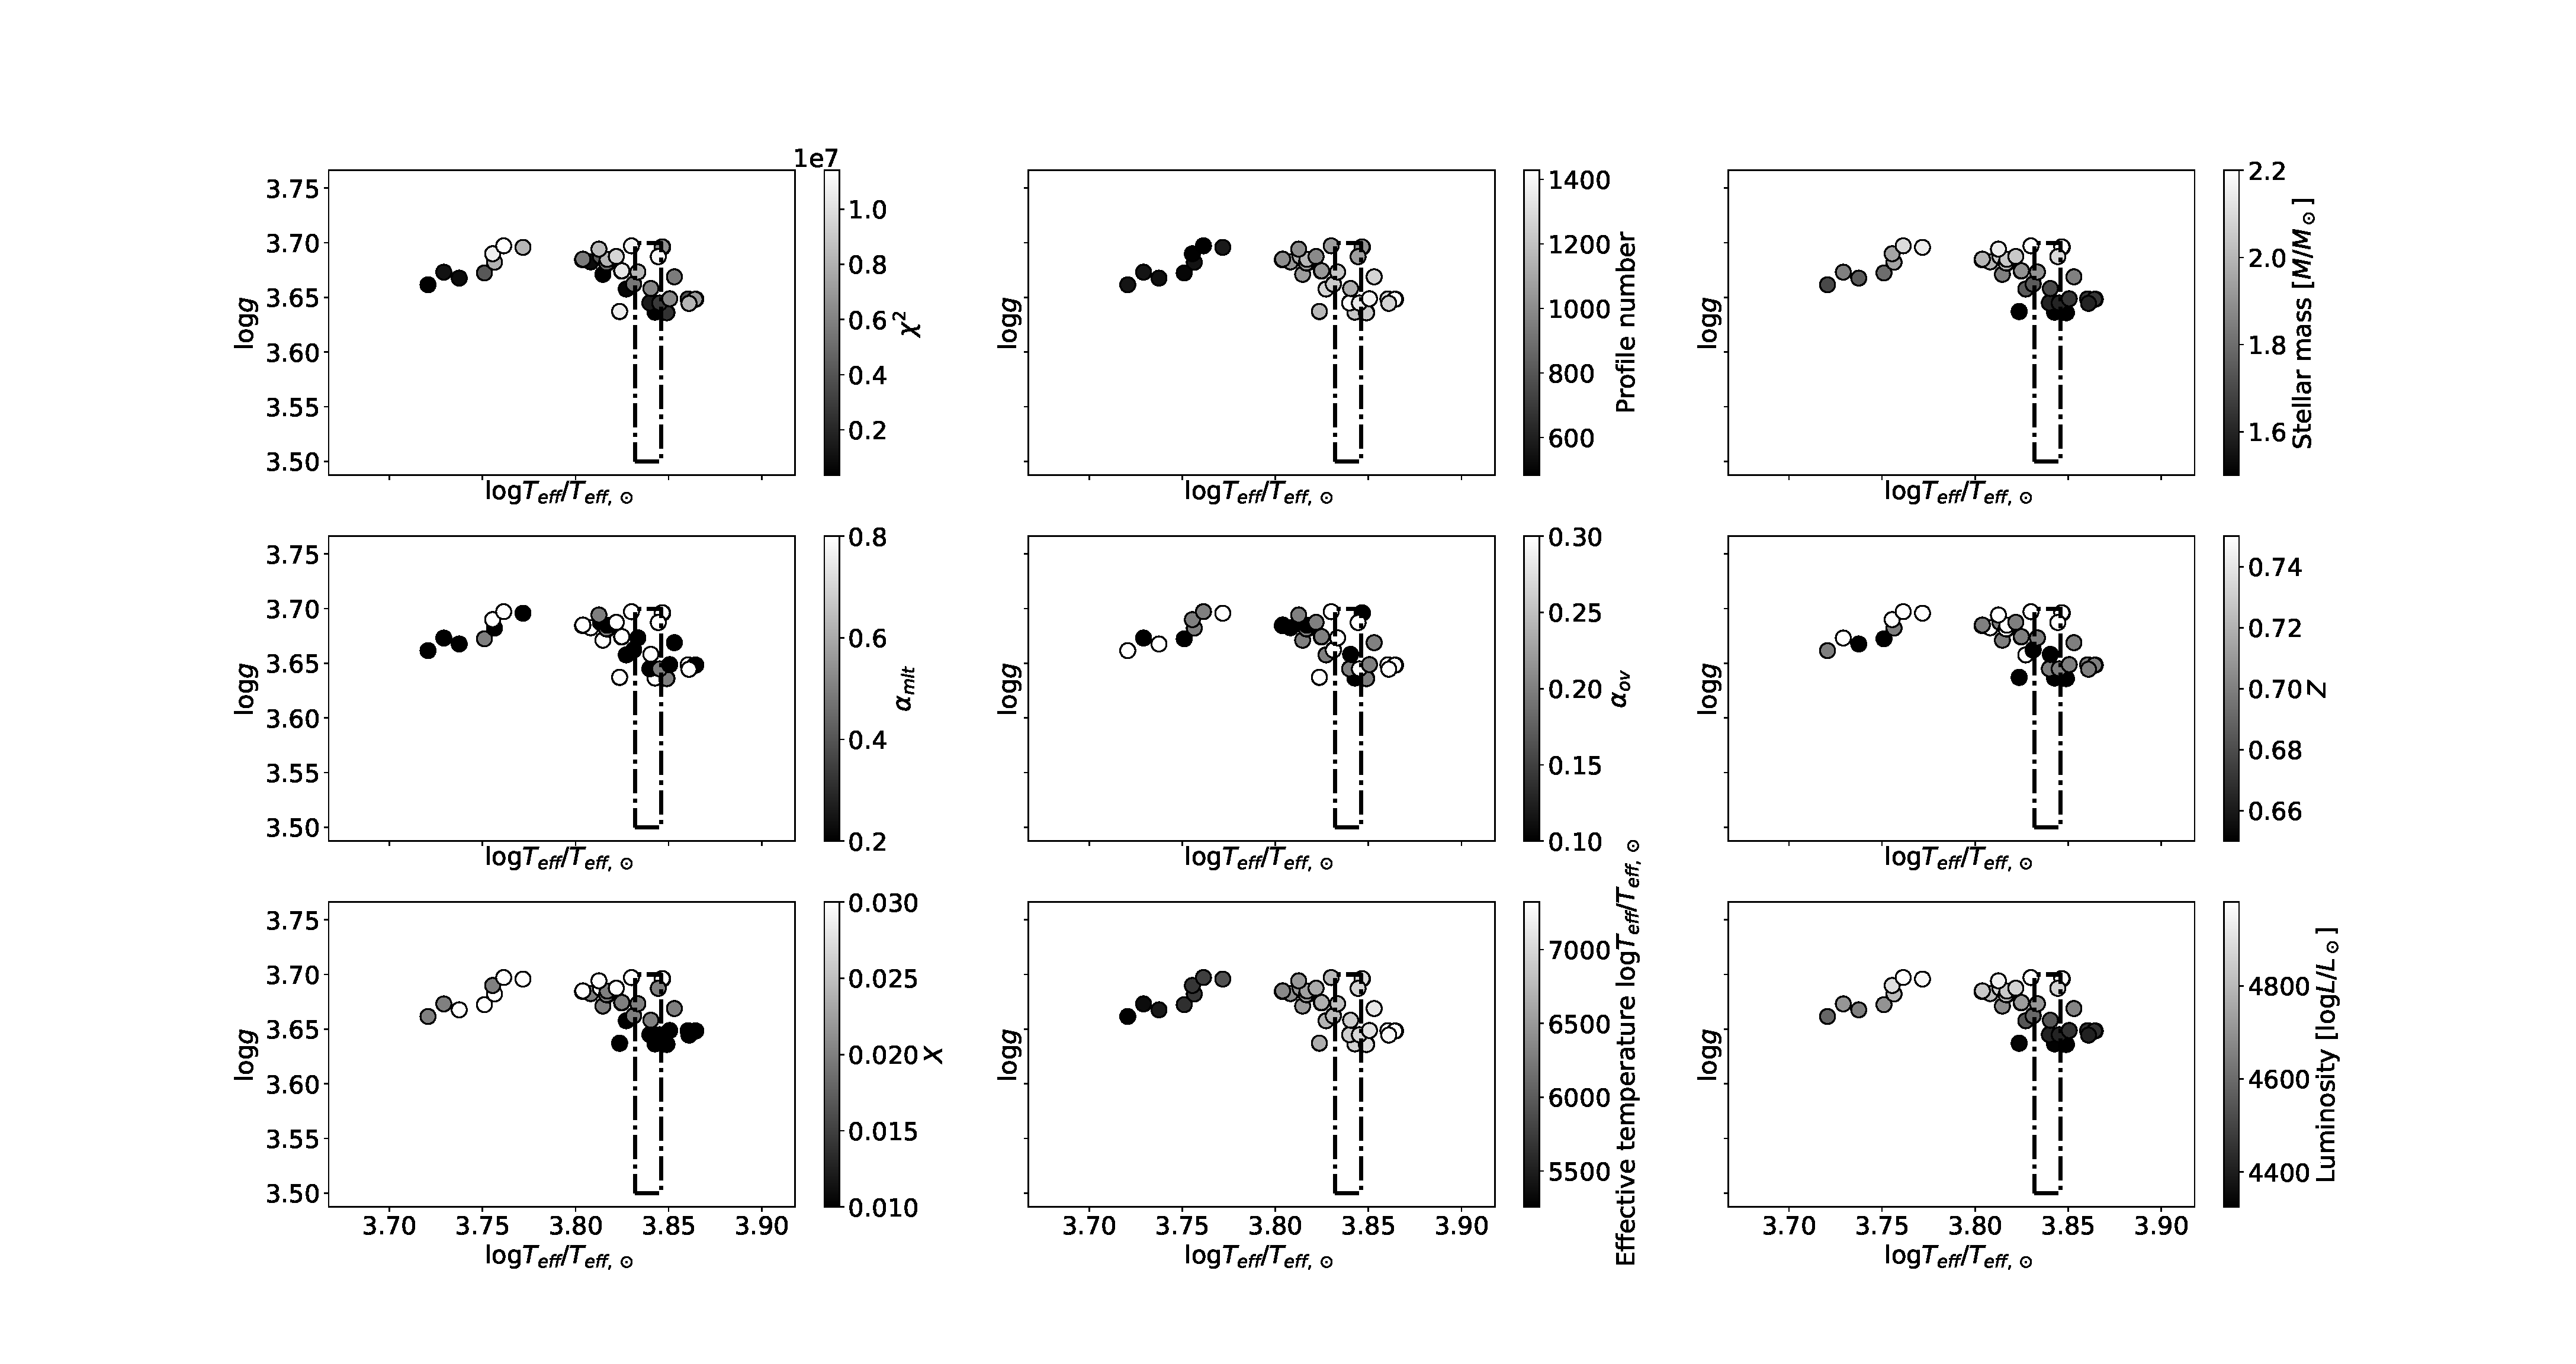
\includegraphics[width=1\textwidth]{scatter_all_v2.eps}
	\makebox[\textwidth][c]{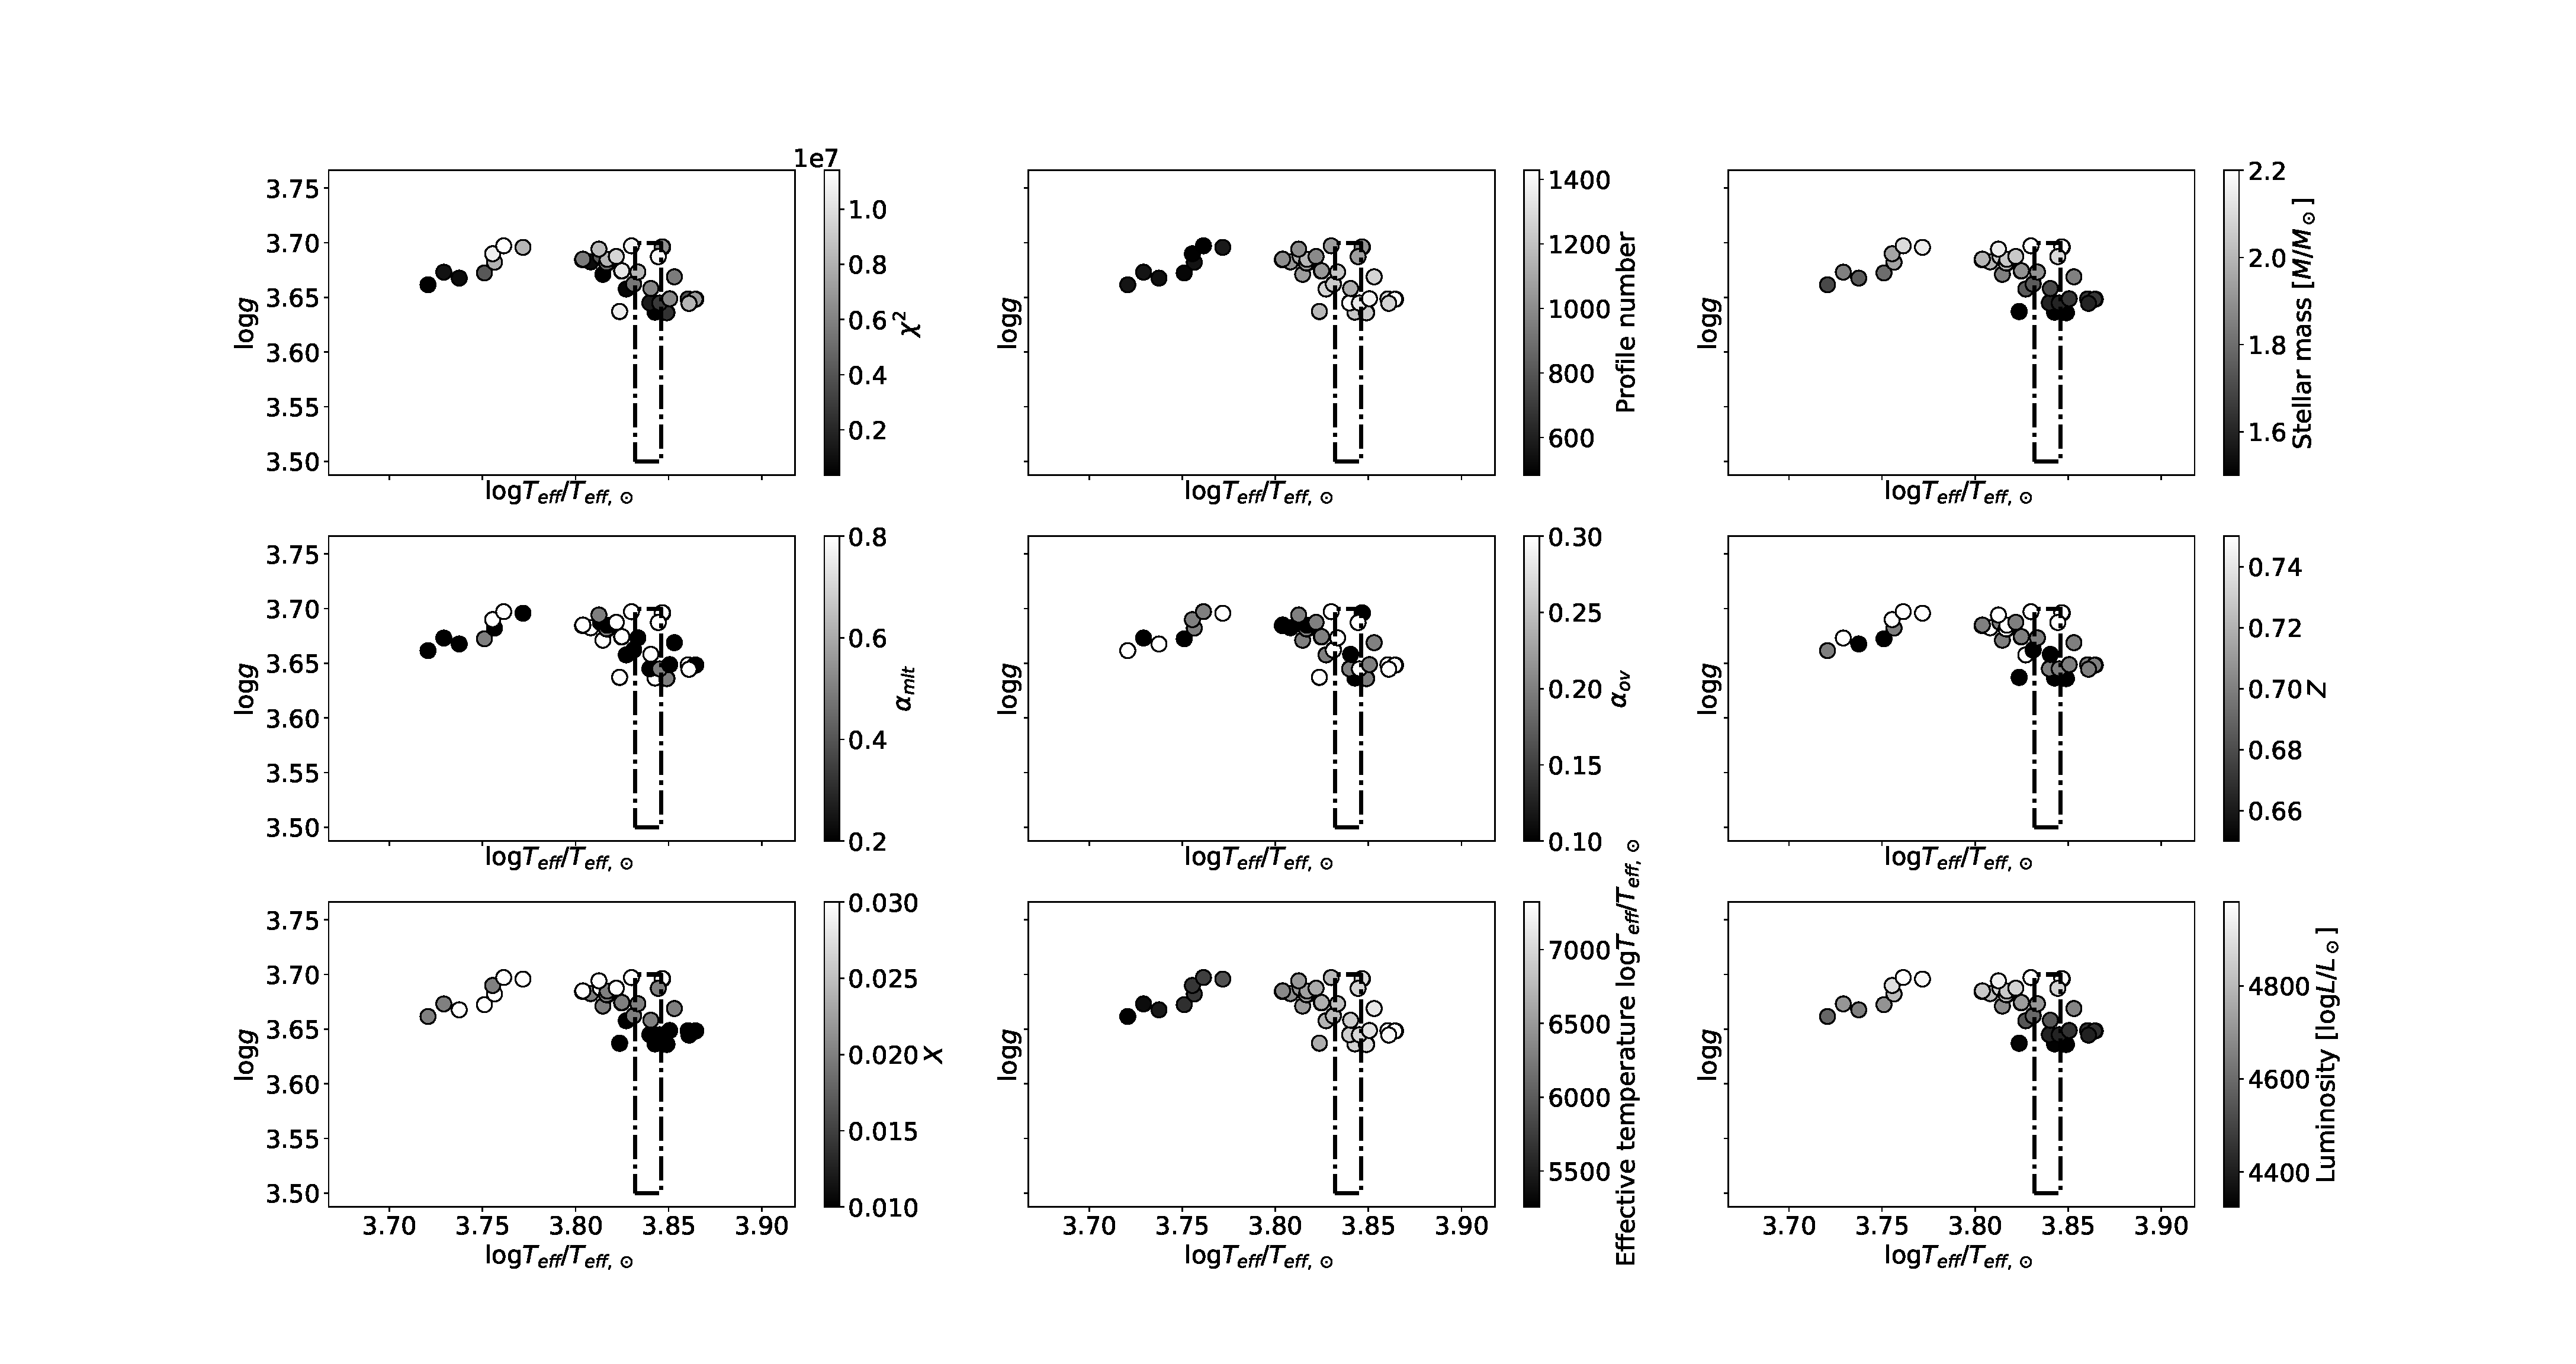
\includegraphics[width=1.5\textwidth]{scatter_all_v2.eps}}%
	\caption{Scatter plots showing \teff, \logg color coded with nine different parameters for the 5\% best models (without resolution control). The plots color coded with \teff and \logg are plotted to show that the plotting method works correctly. The run was made with the Lenz obsevational parameters set. }
	\label{scatter}
\end{figure}


Here, \logg is plotted as a function of \teff and color coded with the corresponding \chis. The 1$\sigma$ uncertainty on \logg and \teff is marked with a black stippled line. Some of the scatter plots shows expected tendencies such as \l, \logg, \teff and profile numbers. Since higher profile number is at a later stage\footnote{Note that the profile number does only indicate the stage of that individual track i.e profile number 900 on one tracks is not necessarily at the same stage for the same profile number on a different track. }, the effective temperature is much lower for lower profile numbers. There is a gap in models around \teff = 3.79 in the 5\% selection criteria. From the profile number it is also clear that the models distributes into two groups where the lower profile numbers corresponds to those on the pre-ms and the higher profile numbers are ms and thereafter. The pre-ms models will be ignored since they are not as reliable as the rest of the models. This group of models is also significantly further away from the errorbox and they will therefore not affect the main result. 

The lowest \chis linearly seems to linearly decrease with \teff. This is because \logg is strongly related to $\rho$ (hence, $\Delta \nu$ and \teff).  
For the element abundances, there is a trend a that lower values of \logg yield lower values of Z and X, in particular. This falls out of \eqref{meanmol} as high abundances of hydrogen and/or metallicity causes a lower mean molecular weight. Since $\mu \propto \rho \propto g$, a smaller value of X or Z yields a smaller value for g as well. Since $g$ is also directly proportional to the mass, the mass decreases with \logg in the plot as well. 

There seems to be no recognizable  in the $\alpha_{mlt}$ and $\alpha_{ov}$ color coding. Since there is a definite correlation between the convection and structure of the star, it would be expected to see a trend between the mixing length or overshoot parameter and \logg and \teff. Since this sample is small, it cannot be excluded that there is a trend that can be found if mode data points were included.   


\subsubsection{l=0,1,2 modes}
A new calculation was conducted in GYRE for l=0, l=1 and l=2 modes for all of these models. The frequencies produced gives a further constrain of the best models as all frequencies can now be compared with observations. Since mode identification is not complete for 44 Tau the radial n,l,m for the frequencies are not finally determined. Therefore they cannot be compared to the individual frequencies calculated in the model without first giving an estimated guess on the n,l and m. Therefore a calculation is conducted based on the fact that n,l and m is known for the models. To ensure that the \chis are comparable between each model, as mentioned earlier, the models all need to have the same amount of fitting parameters. This is not an issue in the first \chis calculations with l=0, since the initial \chis is only based on the same two frequencies for all models. But for l=1 and l=2 the picture is less simple as the number of fitting parameters may vary from model to model, unless it is taken into consideration. The first way to do so is to weight each frequency individually and take the likelihood into account. Though this method probably provides a more detailed and statistically stringent result, it is does require a  very thorough estimate and evaluation of the single frequencies. This is beyond the scope of this work, and instead it is therefore made sure in the way the code is constructed, that this can only be an issue if the number of theoretically produced frequencies is lower than the observed number 8and this is unlikely to happen as these models have already been sorted out in the first \chis round. 

It is carried out in the following way: for each model, each individual model-frequency is compared to all observed frequencies and the best match (i.e. the smallest difference) is thereby assumed to be the closest frequency. This is repeated from the lowest to highest frequency until all model-frequencies has been given a best match observation frequency. This means that the observed frequency will be given the n.l and m of the best -matching model-frequency. Each model then has an estimated set of frequencies where \chis can be computed. This off course does not take into consideration that some frequencies have an estimated radial order and spherical degree. Nor does it take into consideration that the radial fundamental mode and first overtone are already determined (and might match it to n that are higher, however these models should be excluded as their match will not be good if the two first frequencies do not match expectations). This yields a \chis 

\begin{align}
\chi^2 &= \left(\frac{\nu_{\text{all,obs}}^i-\nu^i_{\text{all,theo}}}{\sigma^i_{\text{first}}}\right)^2
 +
         \left(\frac{\text{T}_\text{eff,obs}^i-\text{T}_\text{eff,theo}^i}{\sigma^i_{\text{T}_\text{eff}}}\right)^2  \nonumber \\
  & \quad +
\left(\frac{\log \text{g}_\text{obs}^i-\log \text{g}_\text{theo}^i}{\sigma^i_{\log \text{g}}}\right)^2  + \left(\frac{\log \text{L}_\text{obs}^i-\log \text{L}_\text{theo}^i}{\sigma^i_{\log \text{L}}}\right)^2, 
 \label{eq:chis_all}
\end{align}

From these, the models with the lowest \chis is found for the two different luminosities respectively. . 

\subsection{Results}
The best models found for different runs of 44 Tau are shown in \tabref{bestmodels}. It can here be seen that the variation from GAIA run and Lenz run does not affect the total result. It does however shift the best found model if only including the observational parameters. The reason for this is that the frequencies weigh more in the \chis than the observational parameters. Artificially enhancing the uncertainties on the frequencies does shift the best model, but the total \chis is ...WORSE/BETTER?.

\begin{table}[]
	\begin{tabular}{lllllllllllll}
		profile number & M{[}$M_\odot${]} & X & Z & $\alpha_{mlt}$ & $\alpha_{ov}$ & \textbackslash{}teff & \textbackslash{}logg & \textbackslash{}l & $\chi_{tot}$ & $\chi_{obs_params}$ & $\chi_{freqs}$ & observation set \\
		&                  &   &   &                &               &                      &                      &                   &              &                     &                &                 \\
		&                  &   &   &                &               &                      &                      &                   &              &                     &                &                 \\
		&                  &   &   &                &               &                      &                      &                   &              &                     &                &                 \\
		&                  &   &   &                &               &                      &                      &                   &              &                     &                &                 \\
		&                  &   &   &                &               &                      &                      &                   &              &                     &                &                 \\
		&                  &   &   &                &               &                      &                      &                   &              &                     &                &                 \\
		&                  &   &   &                &               &                      &                      &                   &              &                     &                &                 \\
		&                  &   &   &                &               &                      &                      &                   &              &                     &                &                 \\
		&                  &   &   &                &               &                      &                      &                   &              &                     &                &                 \\
		&                  &   &   &                &               &                      &                      &                   &              &                     &                &                 \\
		&                  &   &   &                &               &                      &                      &                   &              &                     &                &                 \\
		&                  &   &   &                &               &                      &                      &                   &              &                     &                &                 \\
		&                  &   &   &                &               &                      &                      &                   &              &                     &                &                 \\
		&                  &   &   &                &               &                      &                      &                   &              &                     &                &                 \\
		&                  &   &   &                &               &                      &                      &                   &              &                     &                &                 \\
		&                  &   &   &                &               &                      &                      &                   &              &                     &                &                 \\
		&                  &   &   &                &               &                      &                      &                   &              &                     &                &                 \\
		&                  &   &   &                &               &                      &                      &                   &              &                     &                &                 \\
		&                  &   &   &                &               &                      &                      &                   &              &                     &                &                 \\
		&                  &   &   &                &               &                      &                      &                   &              &                     &                &                 \\
		&                  &   &   &                &               &                      &                      &                   &              &                     &                &                 \\
		&                  &   &   &                &               &                      &                      &                   &              &                     &                &                 \\
		&                  &   &   &                &               &                      &                      &                   &              &                     &                &                 \\
		&                  &   &   &                &               &                      &                      &                   &              &                     &                &                 \\
		&                  &   &   &                &               &                      &                      &                   &              &                     &                &                 \\
		&                  &   &   &                &               &                      &                      &                   &              &                     &                &                 \\
		&                  &   &   &                &               &                      &                      &                   &              &                     &                &                 \\
		&                  &   &   &                &               &                      &                      &                   &              &                     &                &                 \\
		&                  &   &   &                &               &                      &                      &                   &              &                     &                &                 \\
		&                  &   &   &                &               &                      &                      &                   &              &                     &                &                 \\
		&                  &   &   &                &               &                      &                      &                   &              &                     &                &                 \\
		&                  &   &   &                &               &                      &                      &                   &              &                     &                &                 \\
		&                  &   &   &                &               &                      &                      &                   &              &                     &                &                 \\
		&                  &   &   &                &               &                      &                      &                   &              &                     &                &                 \\
		&                  &   &   &                &               &                      &                      &                   &              &                     &                &                 \\
		&                  &   &   &                &               &                      &                      &                   &              &                     &                &                 \\
		&                  &   &   &                &               &                      &                      &                   &              &                     &                &                 \\
		&                  &   &   &                &               &                      &                      &                   &              &                     &                &                 \\
		&                  &   &   &                &               &                      &                      &                   &              &                     &                &                 \\
		&                  &   &   &                &               &                      &                      &                   &              &                     &                &                 \\
		&                  &   &   &                &               &                      &                      &                   &              &                     &                &                 \\
		&                  &   &   &                &               &                      &                      &                   &              &                     &                &                 \\
		&                  &   &   &                &               &                      &                      &                   &              &                     &                &                 \\
		&                  &   &   &                &               &                      &                      &                   &              &                     &                &                 \\
		&                  &   &   &                &               &                      &                      &                   &              &                     &                &                 \\
		&                  &   &   &                &               &                      &                      &                   &              &                     &                &                 \\
		&                  &   &   &                &               &                      &                      &                   &              &                     &                &                 \\
		&                  &   &   &                &               &                      &                      &                   &              &                     &                &                 \\
		&                  &   &   &                &               &                      &                      &                   &              &                     &                &                
	\end{tabular}
	\caption{text}
	\label{bestmodels}
\end{table}
The best model results for the Lenz parameter run can be seen on \figref{hrd44taulenz}. The hrd shows the tracks for masses $M = 1.5,1.6,1.7,1.8,1.9,2.0,2.0$ with the combination of $X$ = $Z=$, $\alpha_{mlt}$, $\alpha_{ov}$. The best total model is marked with a cyan blue dot, on the track marked with red. The green points shows the best 5\% models if the criteria is the total \chis\footnote{The total \chis is the \chis from all frequencies, including $l=1$ and $l=2$ modes plus the \chis from observational parameters.}. Blue dots are the 5\% best models if only observational parameters \logg, \teff, \l is included in the \chis, whereas the red dots is the 5\% if the \chis is only calculated from the frequency fits. The green tracks shows the best track with the black dot marking the best model if the frequency uncertainties have been artificially enhanced as in \eqref{sigma}. This track has the parameter combination of $M = 1.5,1.6,1.7,1.8,1.9,2.0,2.0$ with the combination of $X$ = $Z=$, $\alpha_{mlt}$, $\alpha_{ov}$. 

The green points tend to overlap the red points, which indicates that the frequencies are highly more weighted than the observational parameters. The frequencies thereby controls the final outcome, explaining why there is no difference in the main result by changing between GAIA or Lenz observations. The best 5\% models from frequencies seems to be divided into two groups whereas the group near lower temperatures are models on the pre-ms. Since the pre-ms models were loaded from pre-calculated models as discussed in \chapref{compute}, causing different relaxation of the models, the pre-ms and particularly the frequencies on the pre-ms should not be trusted. Since the best model is between the other group it does not make a difference for the main result, but if further tests should be done with the 5\%, they should be excluded from the sample. 

The best model is placing 44 Tau on the post-ms shortly after hydrogen exhaustion in the core. It is not within the three-sigma errorbars from the observations (whereas the best model with artificially pumped frequencies is), which is also clear since there are other models that are closer to the observed parameters. However, since the frequencies weigh much more, the overall \chis is lower. The frequency fit can be seen on \figref{freqfit}. Here, the observational frequencies are plotted with dimensionless power on the y-axis. They color-coded are color-coded by the spherical degree as follows: $l=0$ are red, $l=1$ are blue and  $l=2$ are green, with dimensionless powers of 1,2 and 3. The black lines indicate the matched theoretical frequency, and the gray lines at the bottom represents all theoretically produced frequencies. The naming of the frequencies are defined as in \tabref{freqs44tau}. Stippled lines are lines of uncertainty on the frequencies, although these are so small that they are not visible. Since the uncertainty is so small, technically none of the theoretical frequencies are matched within the uncertainties. However, they are all matched within a range of $0.2 d^{-1}$. The red named text are two modes for which mode identification differs from the theoretically predicted with the \chis fitting code for the frequencies. This is for $f_10$ and $f_2$ where the estimated modes from mode identification is $l=2$ and $l=1$, whereas they were here estimated to be $l=1$ and $l=2$, respectively. This could be due to different reasons: 1) The pulsation code does not calculated the theoretically produced frequencies correctly. At this point it is already a well-known issue that the theory behind these type of oscillations does not comply well with observations. \citet{lenz2010delta} was indeed successfull with modeling 44 Tau, but this example is the first one of its kind where all modes where reproduced theoretically. More often, pulsation codes does not match observations. 
2)  The \chis routine used in this project does not match the frequencies correctly, resulting in the spherical degrees to be found incorrectly. As discussed earlier in this chapter, the routine only considers the best match frequency, and does not take spherical degree into account at any point. It only guesses it based on the theoretically produced ones. 
3) Due to the high uncertainty in mode identification, some of the modes have been done incorrectly. This is the more likely scenario since 1) and 2) would probably cause issues for more than two modes, and would not have been able to fit the rest either. There is also strong evidence that some modes could be identified wrongly due to the model dependency of the mode identification. It can be seen on \figref{lenzdiss} that the choice of mixing length affects the mode identification significantly. EXPLAIN FIGURE. These models are based on frozen convection where the mixing length describes the local convection. However, time-dependent convection is needed in order to describe the full picture of convection, and the difference in mode identification is significant \citep{dupret2005time}, (Victoria Antoci 2019, private communication).

\begin{figure}[htbp]
	\centering
	%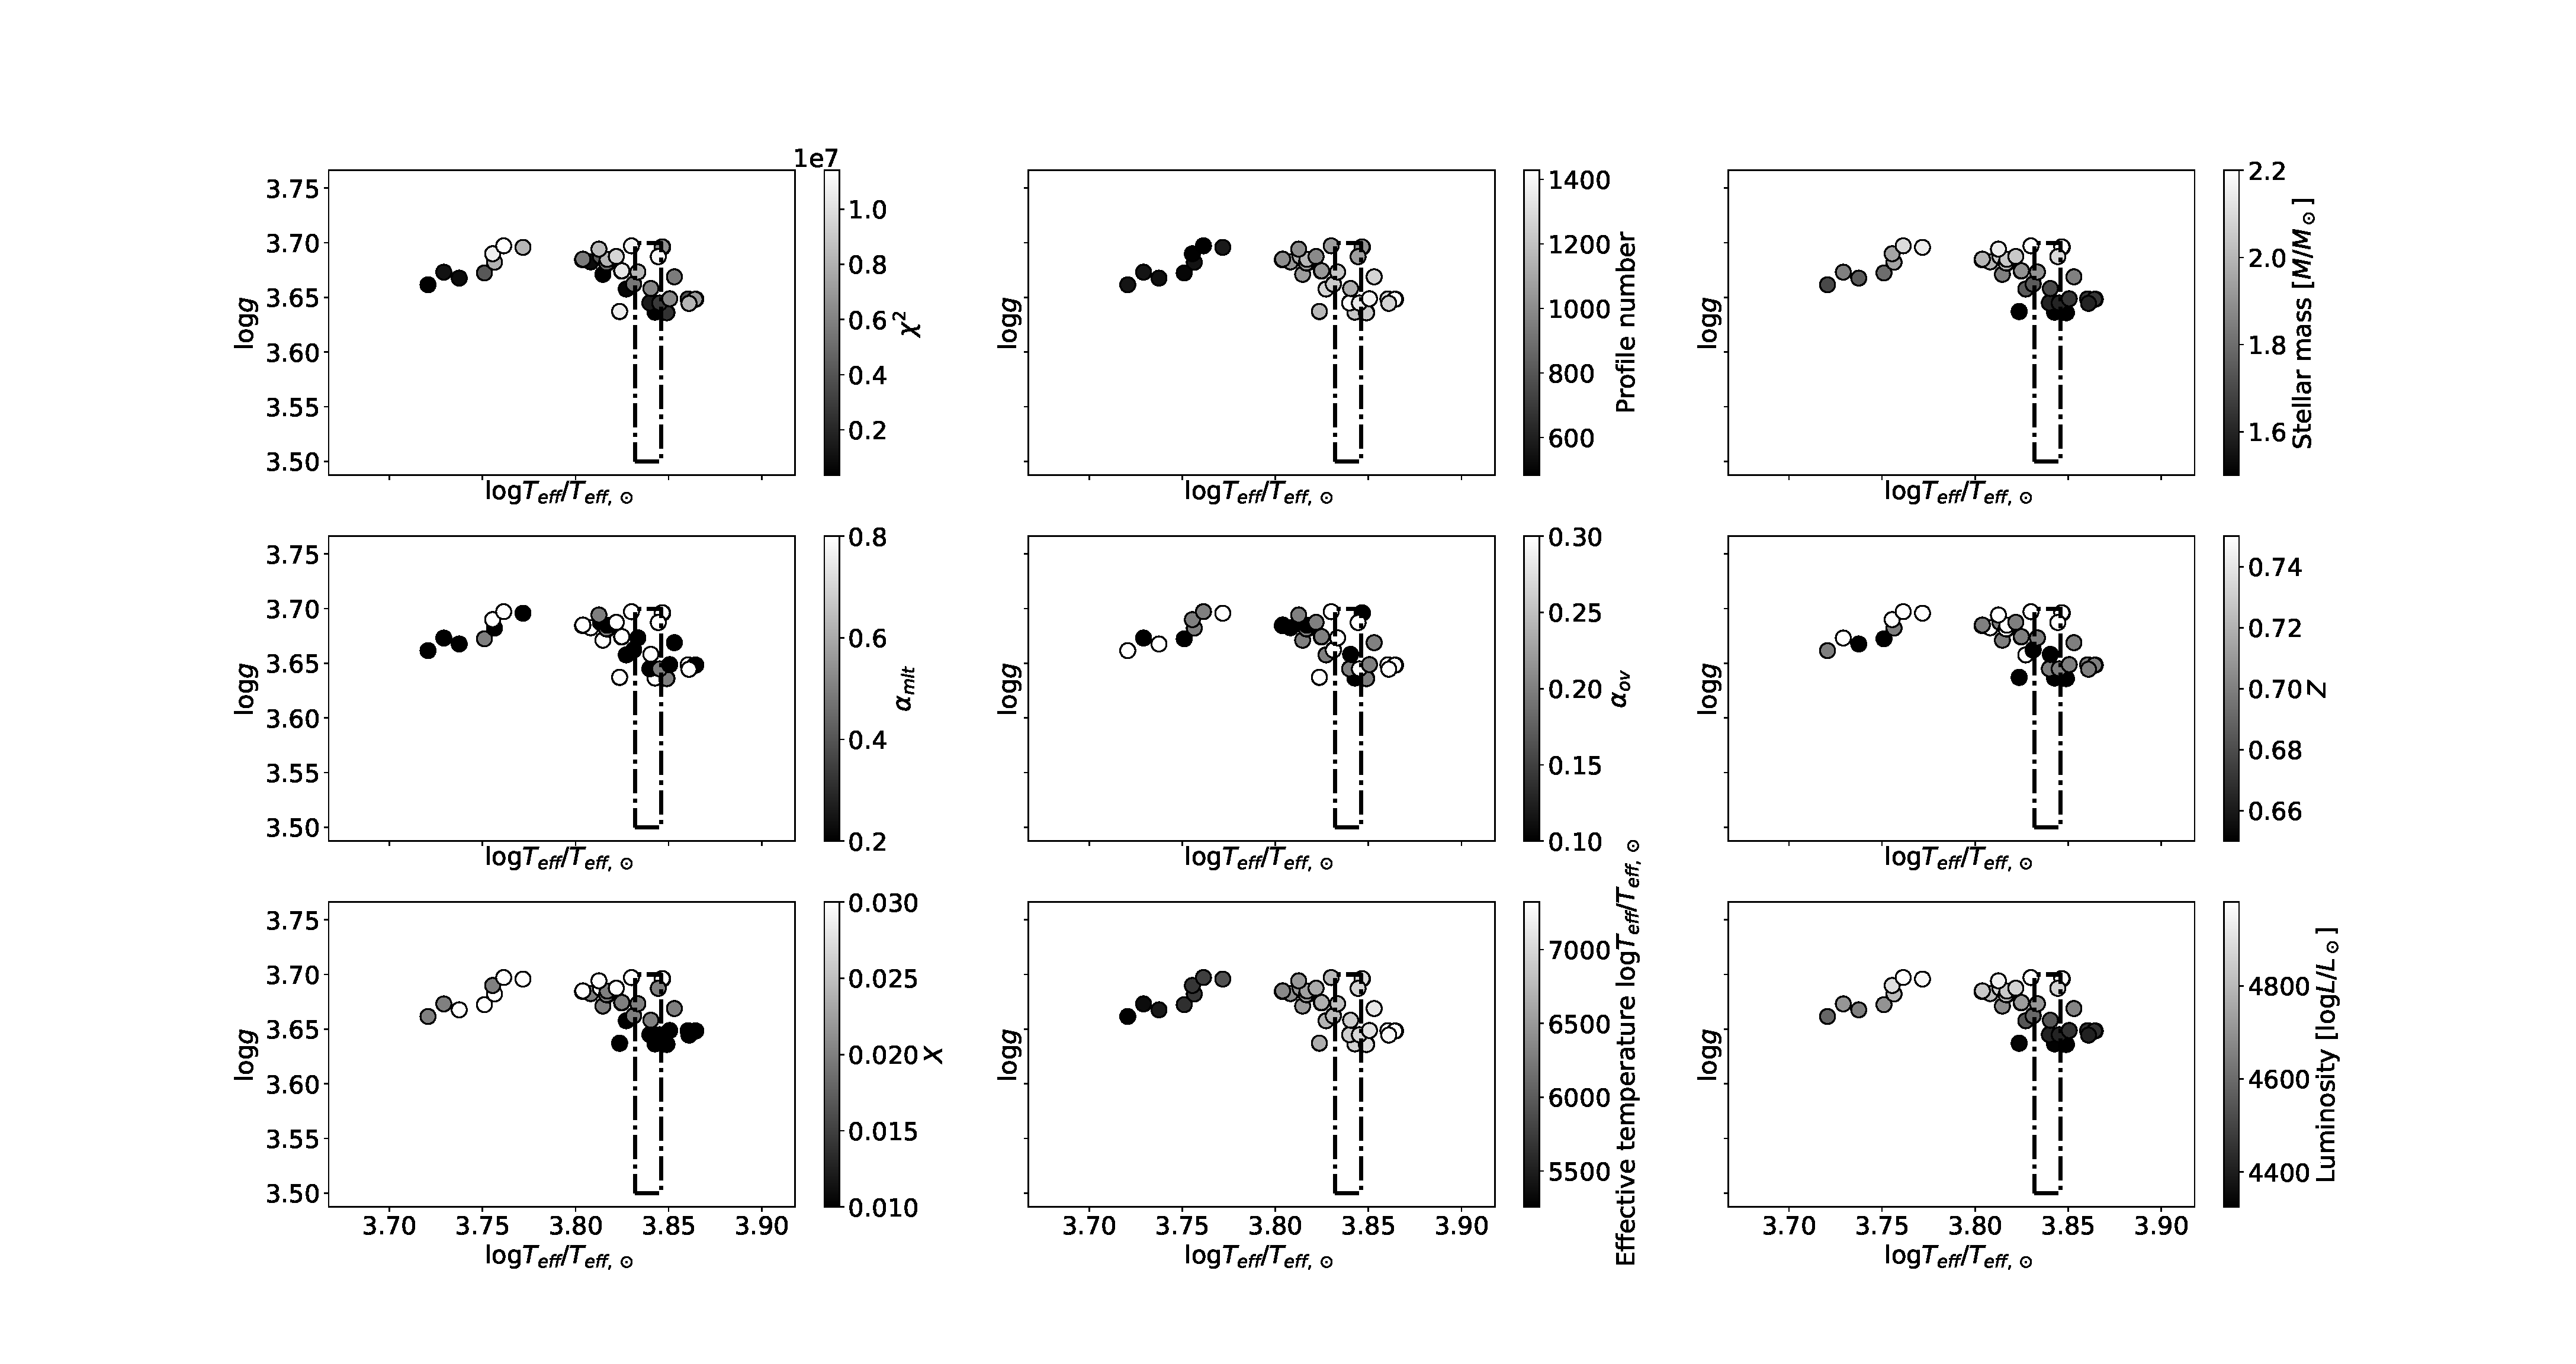
\includegraphics[width=1\textwidth]{scatter_all_v2.eps}
	\makebox[\textwidth][c]{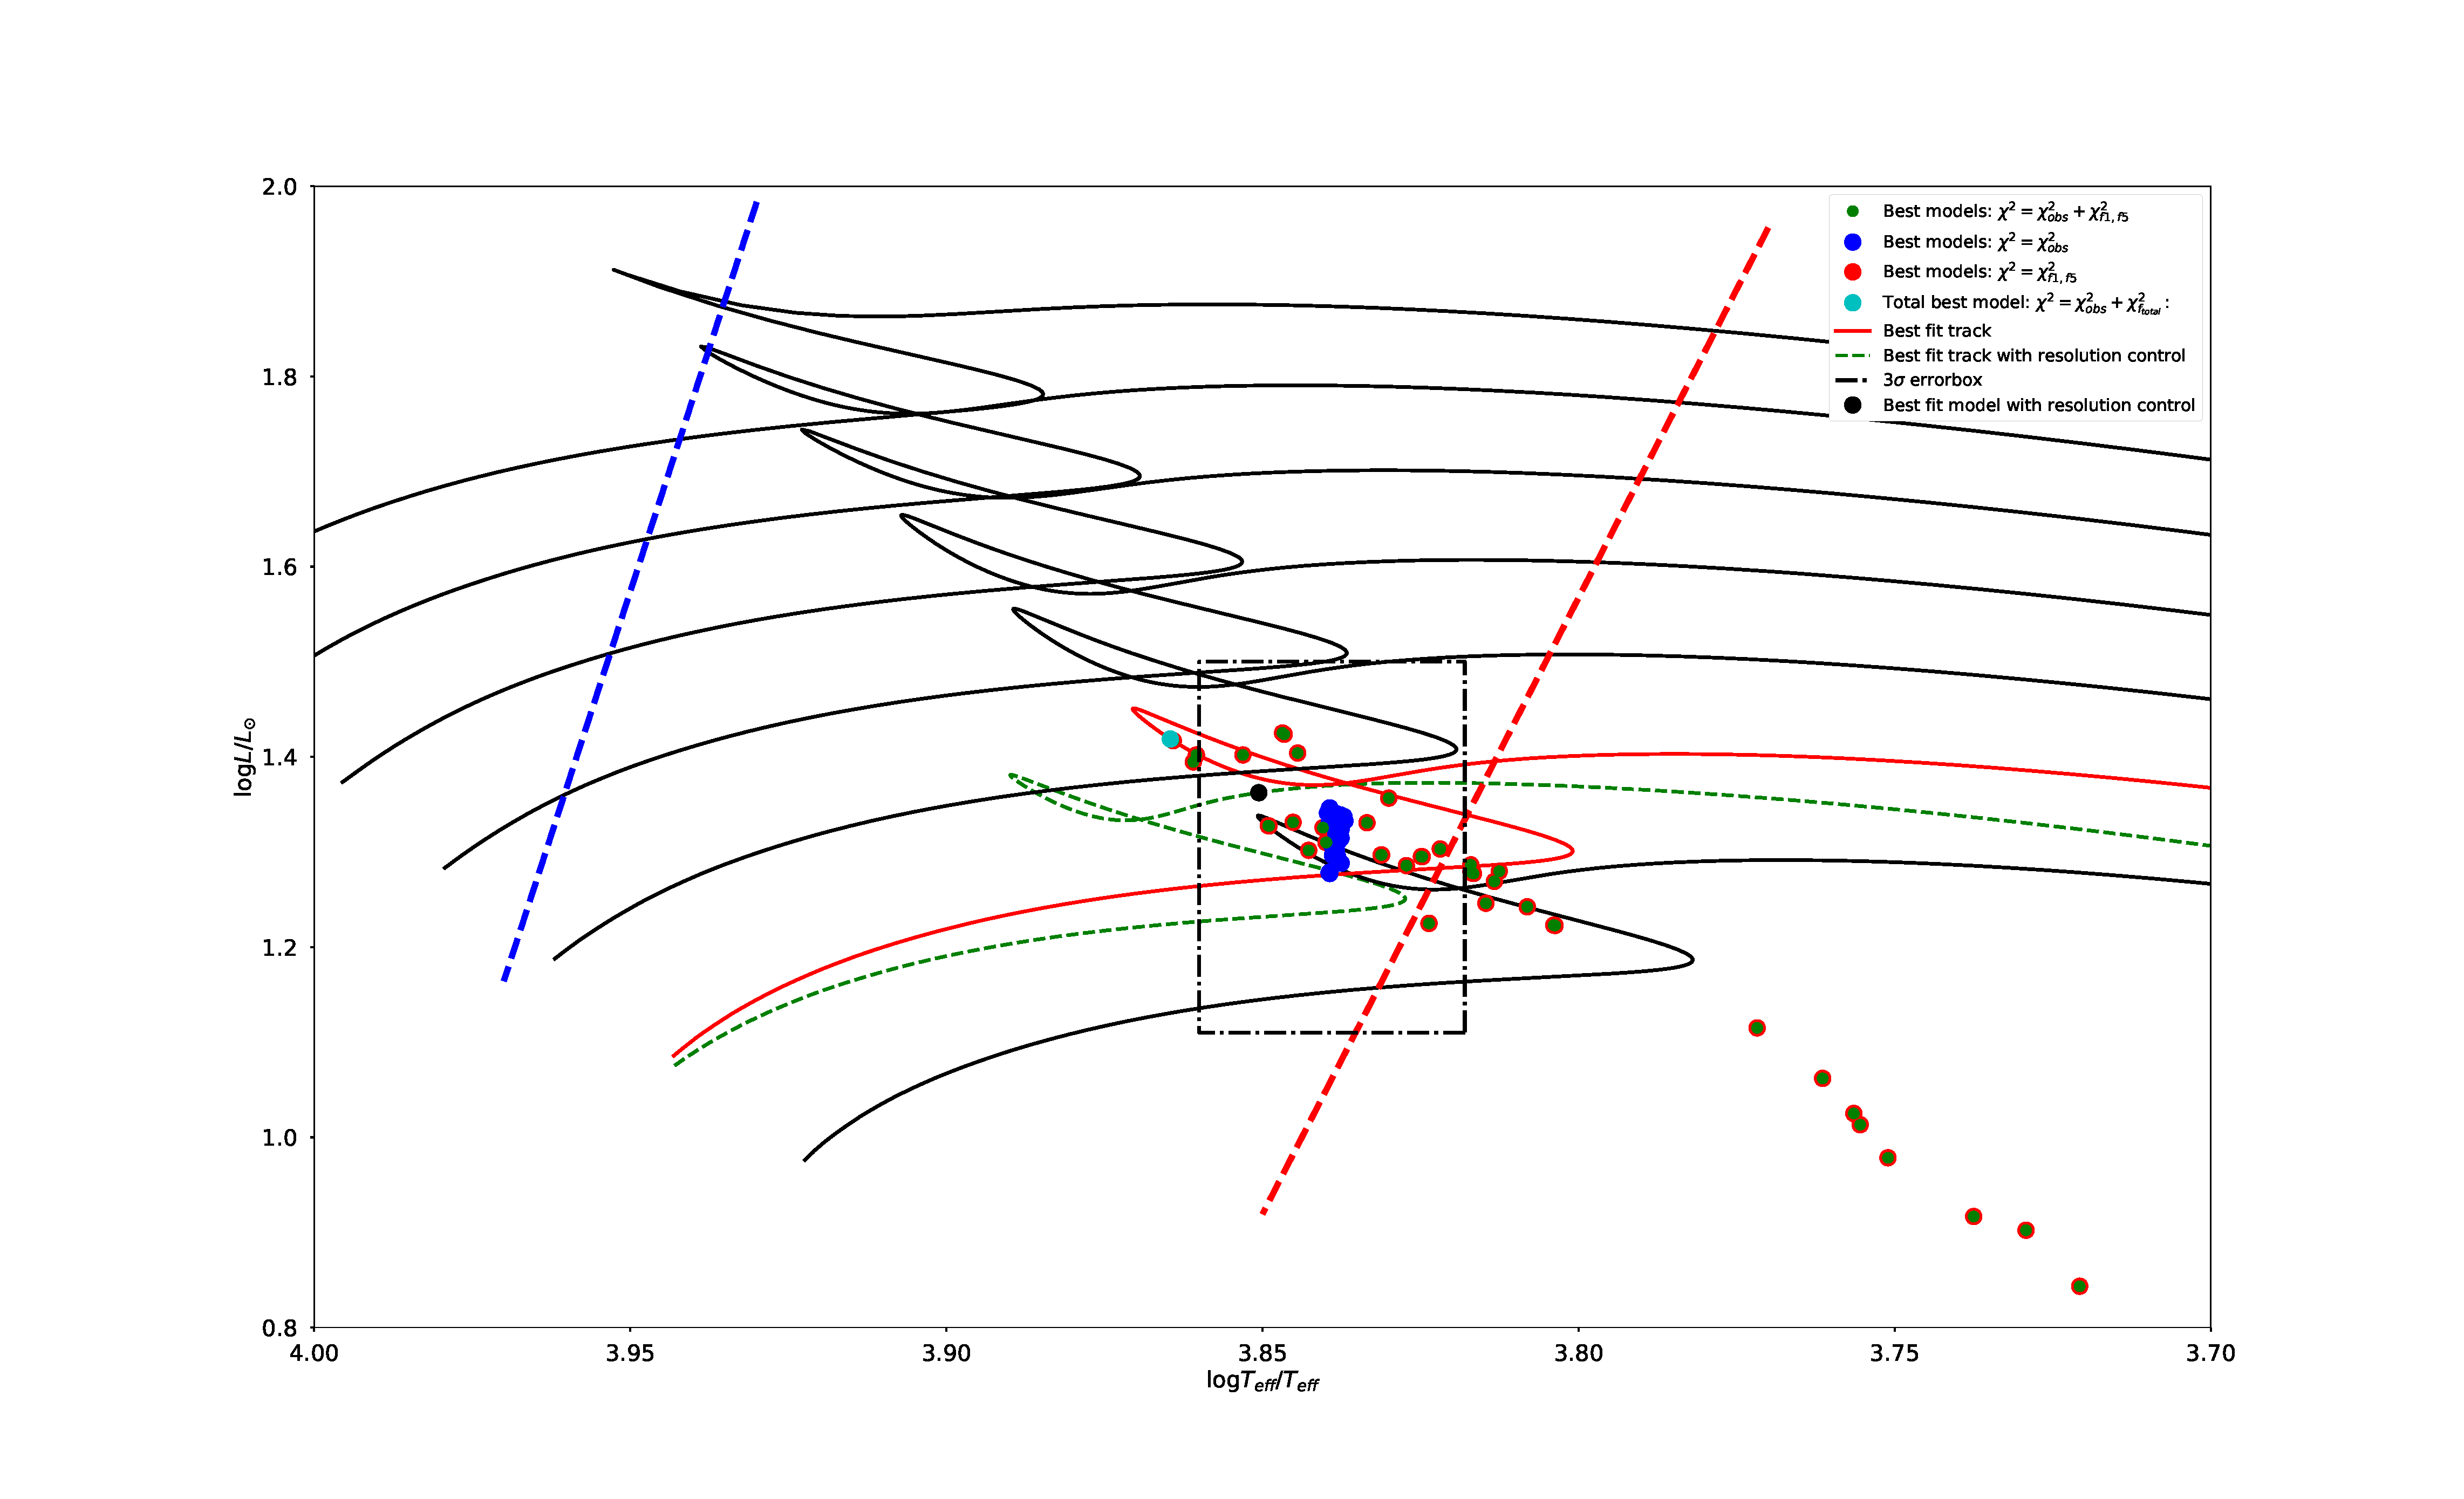
\includegraphics[width=1.5\textwidth]{final_hrd_44tau_lum1.eps}}%
	\caption{}
	\label{hrd44taulenz}
\end{figure}

\begin{figure}[htbp]
	\centering
	%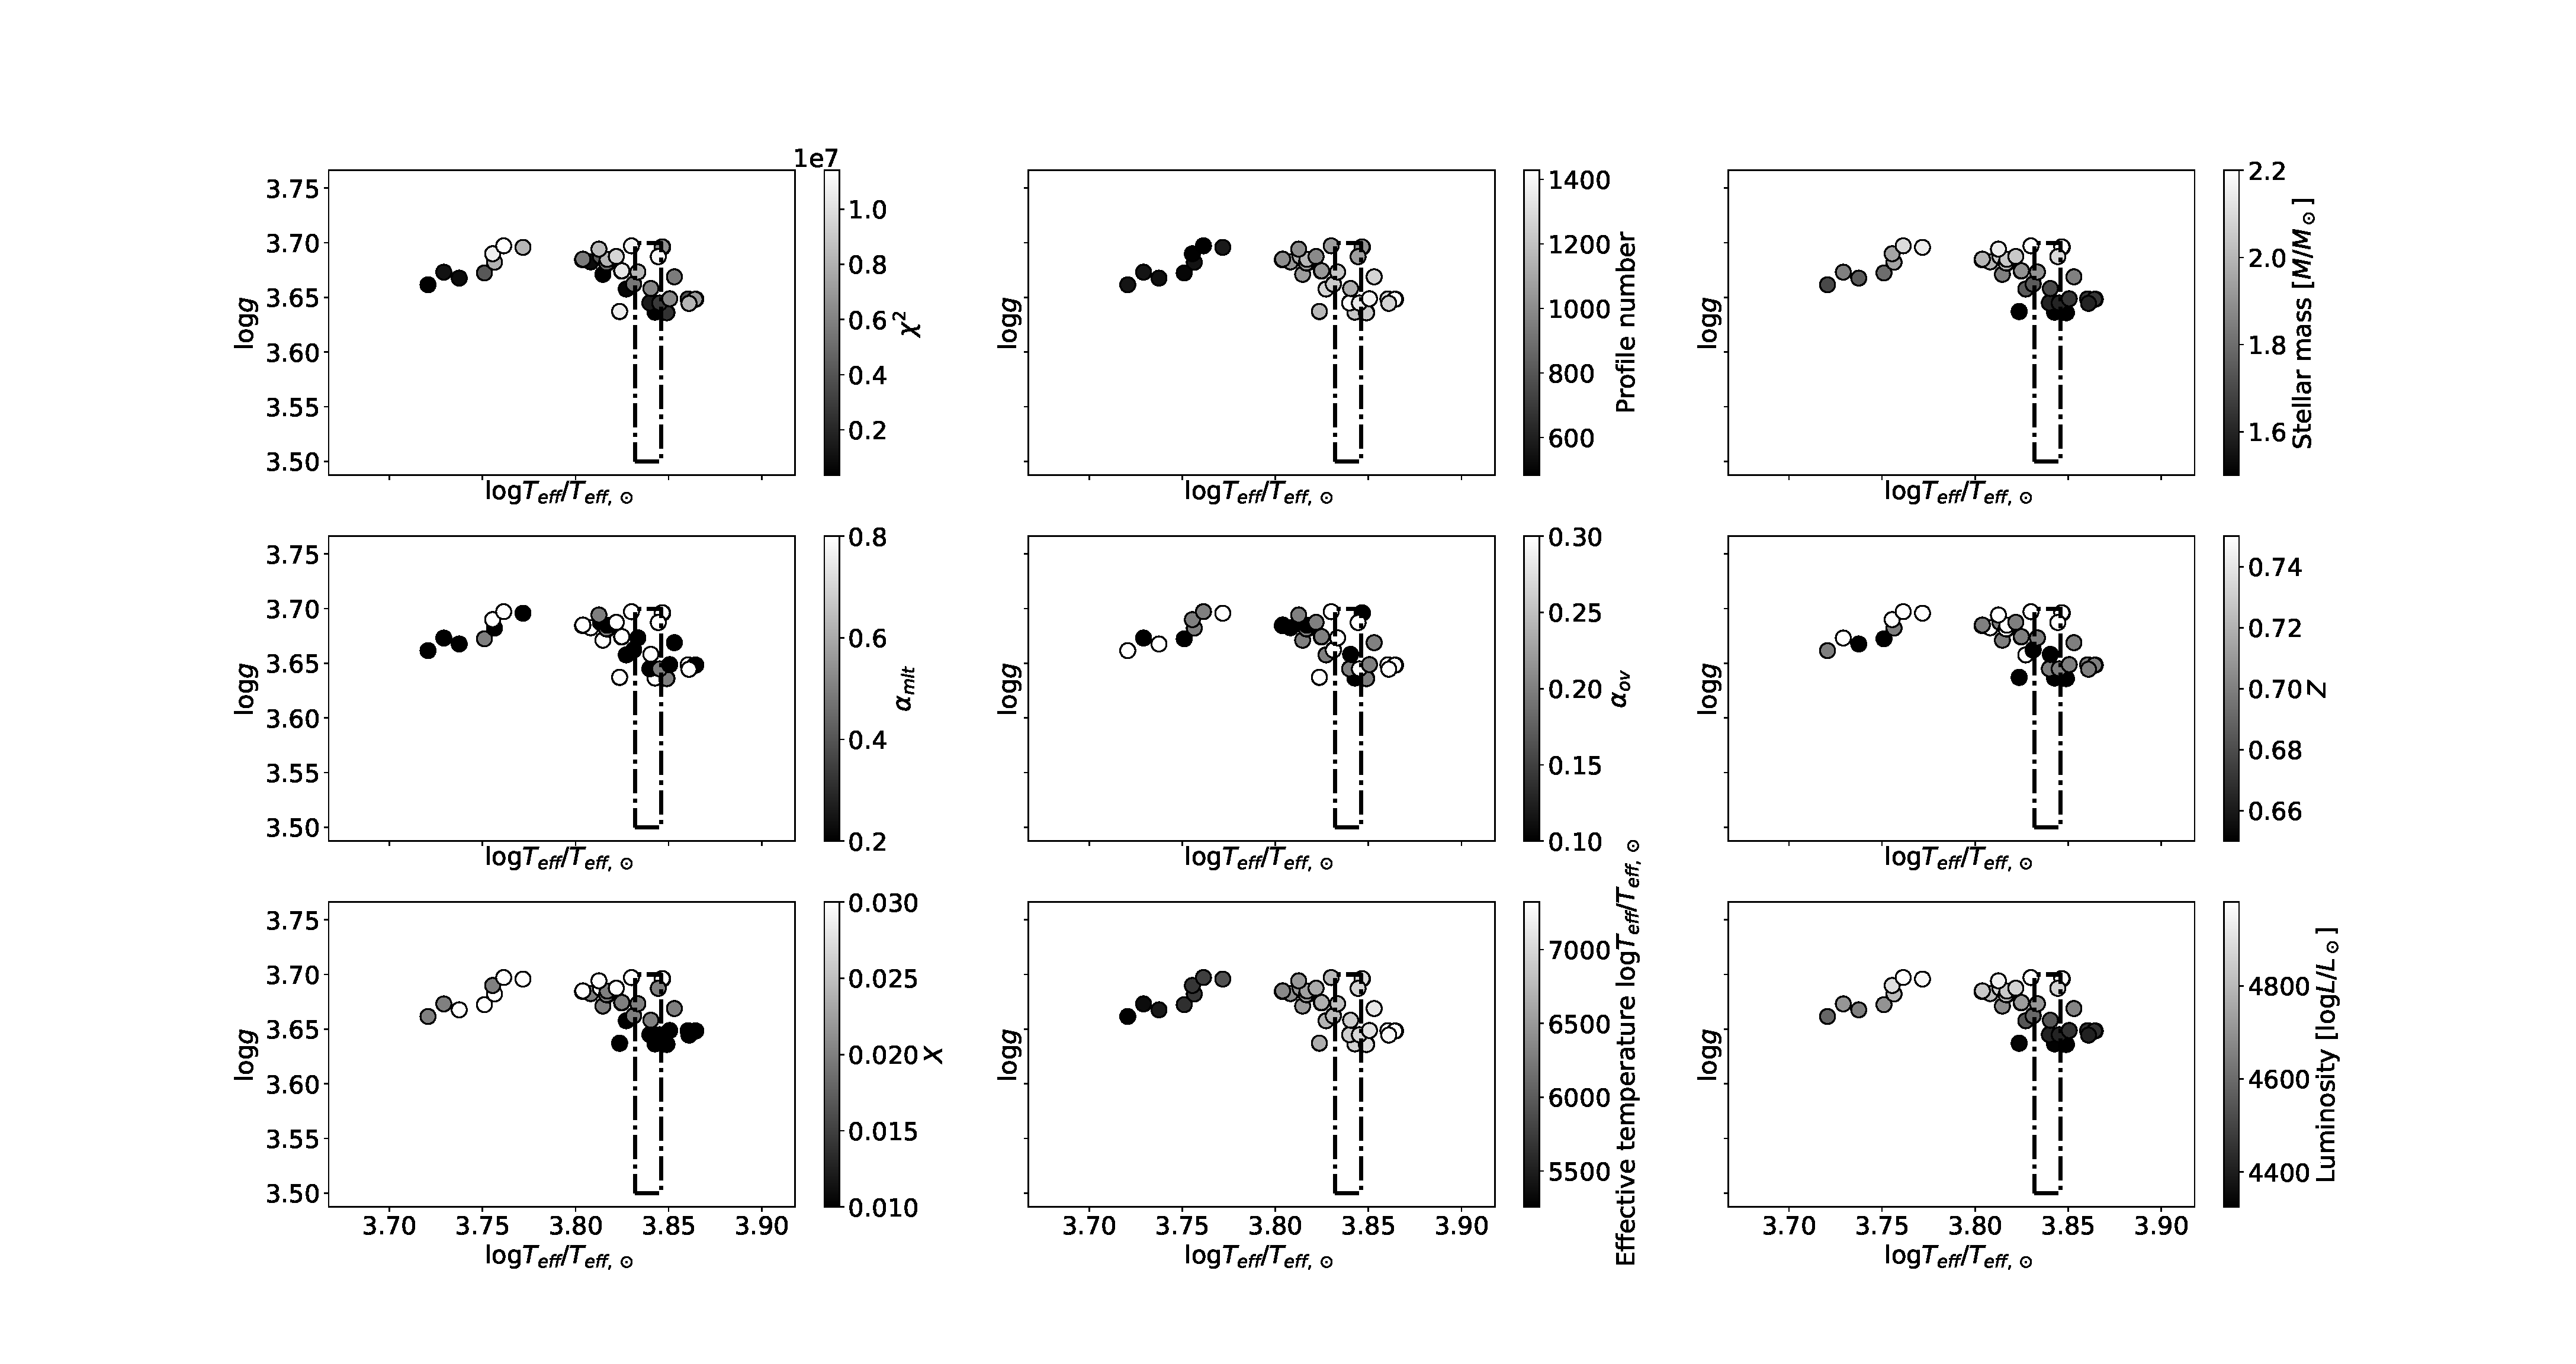
\includegraphics[width=1\textwidth]{scatter_all_v2.eps}
	\makebox[\textwidth][c]{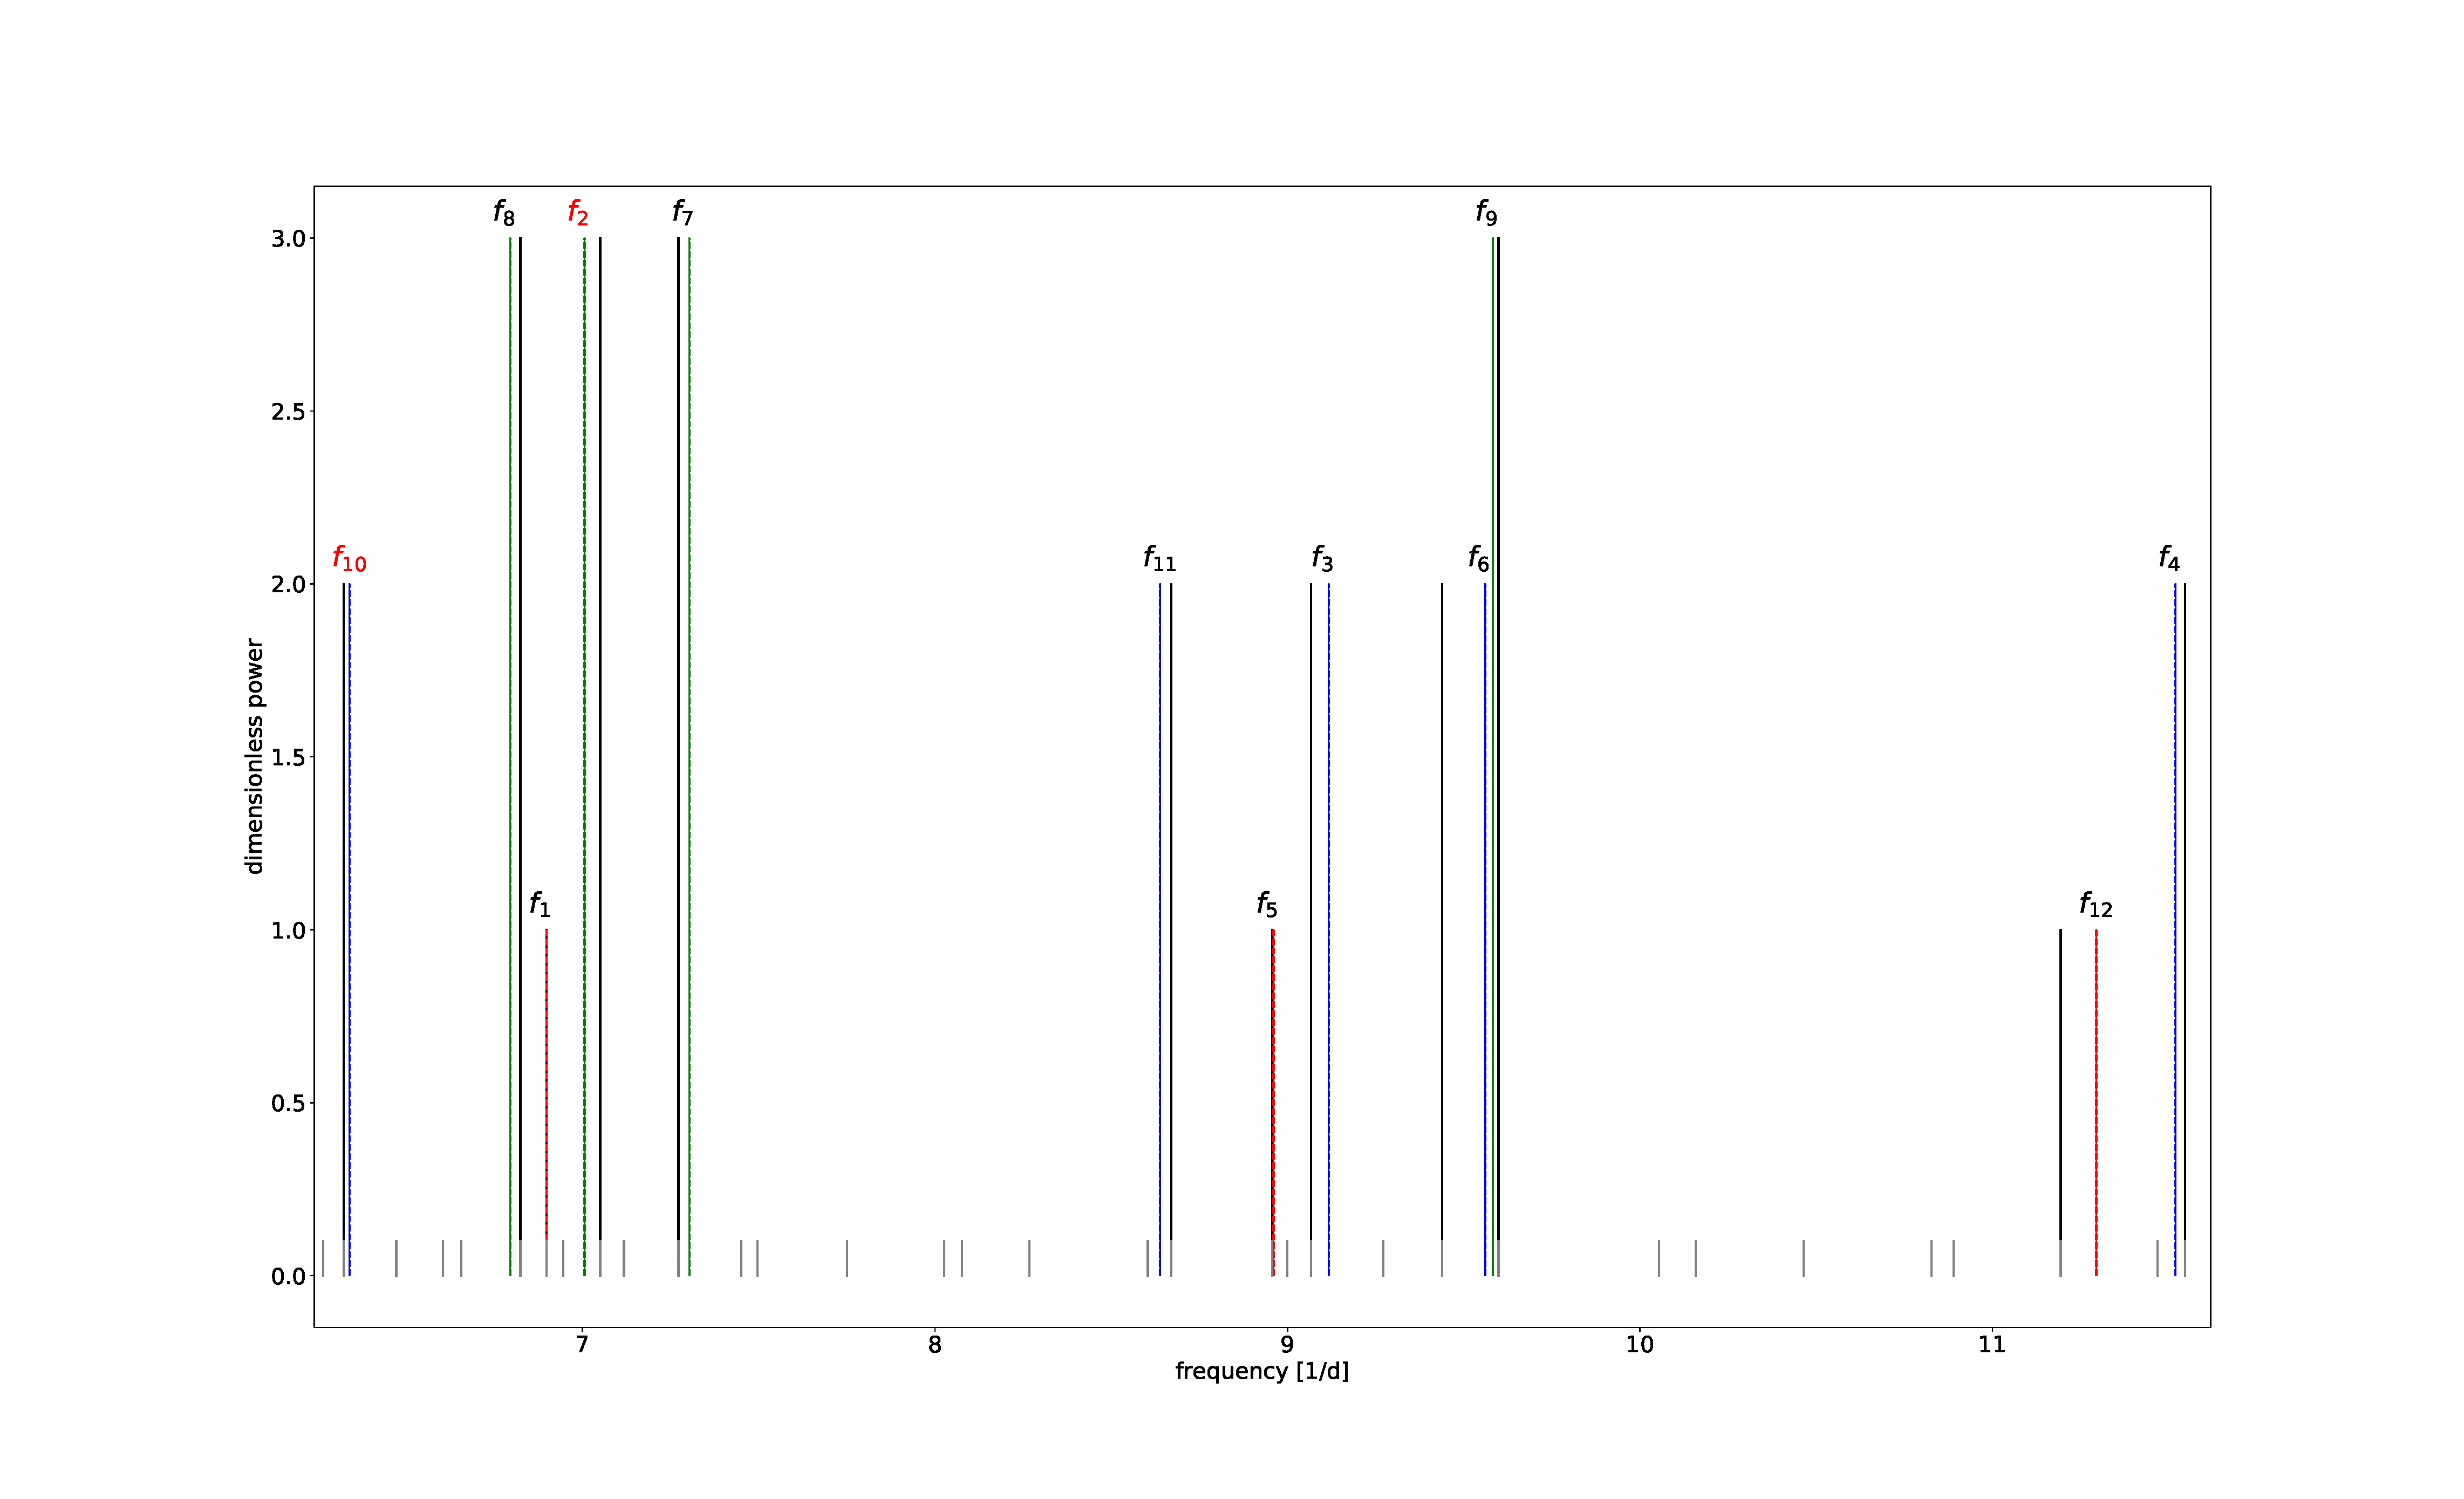
\includegraphics[width=1.5\textwidth]{frequency_fit.eps}}%
	\caption{}
	\label{freqfit}
\end{figure}

\section{Superstar}

On the contrary to 44 Tau, no modes are well enough determined to use an initial constraint for the models of this star. Instead of fitting the frequencies it is therefore more favourable to fit the large frequency separation, introduced in \secref{chap:asteroseismology}. This can be calculated as

\begin{equation}
    \Delta\nu = \nu_{n+1} - \nu_{n},
\end{equation}

\noindent the frequency difference between two (l=0).  The \chis can now be calculated using the observed large frequency separation of 3.5 cycles per day \citep{antoci2014role}, calculated the same way as  \eqref{sigma}, with method one \eqref{sigma}. Employing the standard deviation as \eqref{m2} cannot be done the same way as for 44 Tau since there is only one parameter to sum over. Therefore, the 5\% models with the smallest \chis are found only through the first method, and results are shown shown in \tabref{tab:superstar}.

\begin{table}[htbp]
  \caption{hest}
  \label{tab:superstar}

\begin{tabular}{lllllllllll}
\label{bestchi}
 Model & X & Z & Y & $M[M_\odot]$ & $\alpha_{mlt}$ & $\alpha_{ov}$ & $\log \text{T}_\text{eff}$  & $\log \text{L}$  & $\log \text{g}$ & $\chi^2$ \\
 &  &  &  &  &  &  &  &  &  &  \\
 &  &  &  &  &  &  &  &  &  &  \\
 &  &  &  &  &  &  &  &  &  &  \\
 &  &  &  &  &  &  &  &  &  &  \\
 &  &  &  &  &  &  &  &  &  &  \\
 &  &  &  &  &  &  &  &  &  &  \\
 &  &  &  &  &  &  &  &  &  &  \\
 &  &  &  &  &  &  &  &  &  &  \\
 &  &  &  &  &  &  &  &  &  &  \\
 &  &  &  &  &  &  &  &  &  &  \\
 &  &  &  &  &  &  &  &  &  &  \\
 &  &  &  &  &  &  &  &  &  &  \\
 &  &  &  &  &  &  &  &  &  &  \\
 &  &  &  &  &  &  &  &  &  &  \\
 &  &  &  &  &  &  &  &  &  &  \\
 &  &  &  &  &  &  &  &  &  &  \\
 &  &  &  &  &  &  &  &  &  &  \\
 &  &  &  &  &  &  &  &  &  &  \\
 &  &  &  &  &  &  &  &  &  &  \\
 &  &  &  &  &  &  &  &  &  &  \\
 &  &  &  &  &  &  &  &  &  &  \\
 &  &  &  &  &  &  &  &  &  &  \\
 &  &  &  &  &  &  &  &  &  &  \\
 &  &  &  &  &  &  &  &  &  &  \\
 &  &  &  &  &  &  &  &  &  &  \\
 &  &  &  &  &  &  &  &  &  &  \\
 &  &  &  &  &  &  &  &  &  &  \\
 &  &  &  &  &  &  &  &  &  & 
\end{tabular}
\end{table}

For modes higher than l=0, calculating the \chis for Superstar is significantly more complicated for Superstar, since it is based on the large frequency separation. When l becomes larger than zero, the frequency separation depends significantly on the mixed modes and radial order. Therefore, this part is beyond the scope of this work. 

\subsection{Results}
If HD 187547 is indeed on the pre-me we would expect features from different metallic lines and dust to appear in the spectrum, however no so observations indicate that this should be the case. As mentioned, the pre-ms tracks in \texttt{MESA} made in this work should not be trusted for  the purpose of asteroseismic modeling, since the are all products of the same relaxed pre-calculated pre-ms model. Therefore, the results are forced on to the ms by making a cutoff at profile 900. This is a rough cutoff since profile 900 on one tracks is not necessarily an indication of the same stage for the same profile on another track. A more secure way do it would be to evaluate the helium content in the core and set a limit for the gradient (i.e. defining the ms at a certain limit for an increase in helium in the core). This would however require an individual assessment of each track, and is therefore beyond the scope of this work. 

The issues with modeling HD 187547 compared to 44 Tau are still very much up for discussion. The very small luminosity measured observationally could be explained if it is still in a vary early stage on the ms. Then we would expect $\delta \nu$ to be significantly larger than $3.5d^(-1)$, more like $7d^(-1)$ from Bedding. However, since the pre-ms tracks made in \texttt{MESA} in this work are not made for modeling purposes, the earlier stages of the ms might be affected as well (due to relaxation issues etc.). For the small frequency separation, the results seems more reliable as the 5\% best models for separation and observations has some overlap, which is not the case for the $\delta \nu = 7$. This could be due to several things: 1) The models are simply not trustworthy at these early stages due to insufficient pre-ms tracks. 2) From the resolution evaluation discussed in \secref{sec:resolution}, it was shown that models have smaller resolution at the early stages. If HD 187547 is indeed at a very early stage on the ms, the models are very far apart at this point, causing a larger gap between models. This does not however explain why there is a missing overlap between separation selected models and observation selected models.
3) More constraints are needed on the frequency calculations. As was shown in \chapref{introduction}, the asymptotic relation is only applicable to $n >> l$. This affects the large frequency separation, since the equidistancy in frequency space is otherwise invalid. The frequencies were calculated in the range of $45d^(-1)$ to $80d^(-1)$ to somewhat avoid this issue. But for younger models the frequency of $45d^(-1)$ might still be at very low radial orders $n$(since younger models have higher frequencies), which causes a bias in the models. A plot of the theoretically produced fundamental mode as a function of evolution is shown on \figref{fundmode}.  The equidistancy is valid only for the part of the plot that is a straight line. This covers a frequency range of .... which is good/bad because....


%\begin{figure}[htbp]
%	\centering
%	%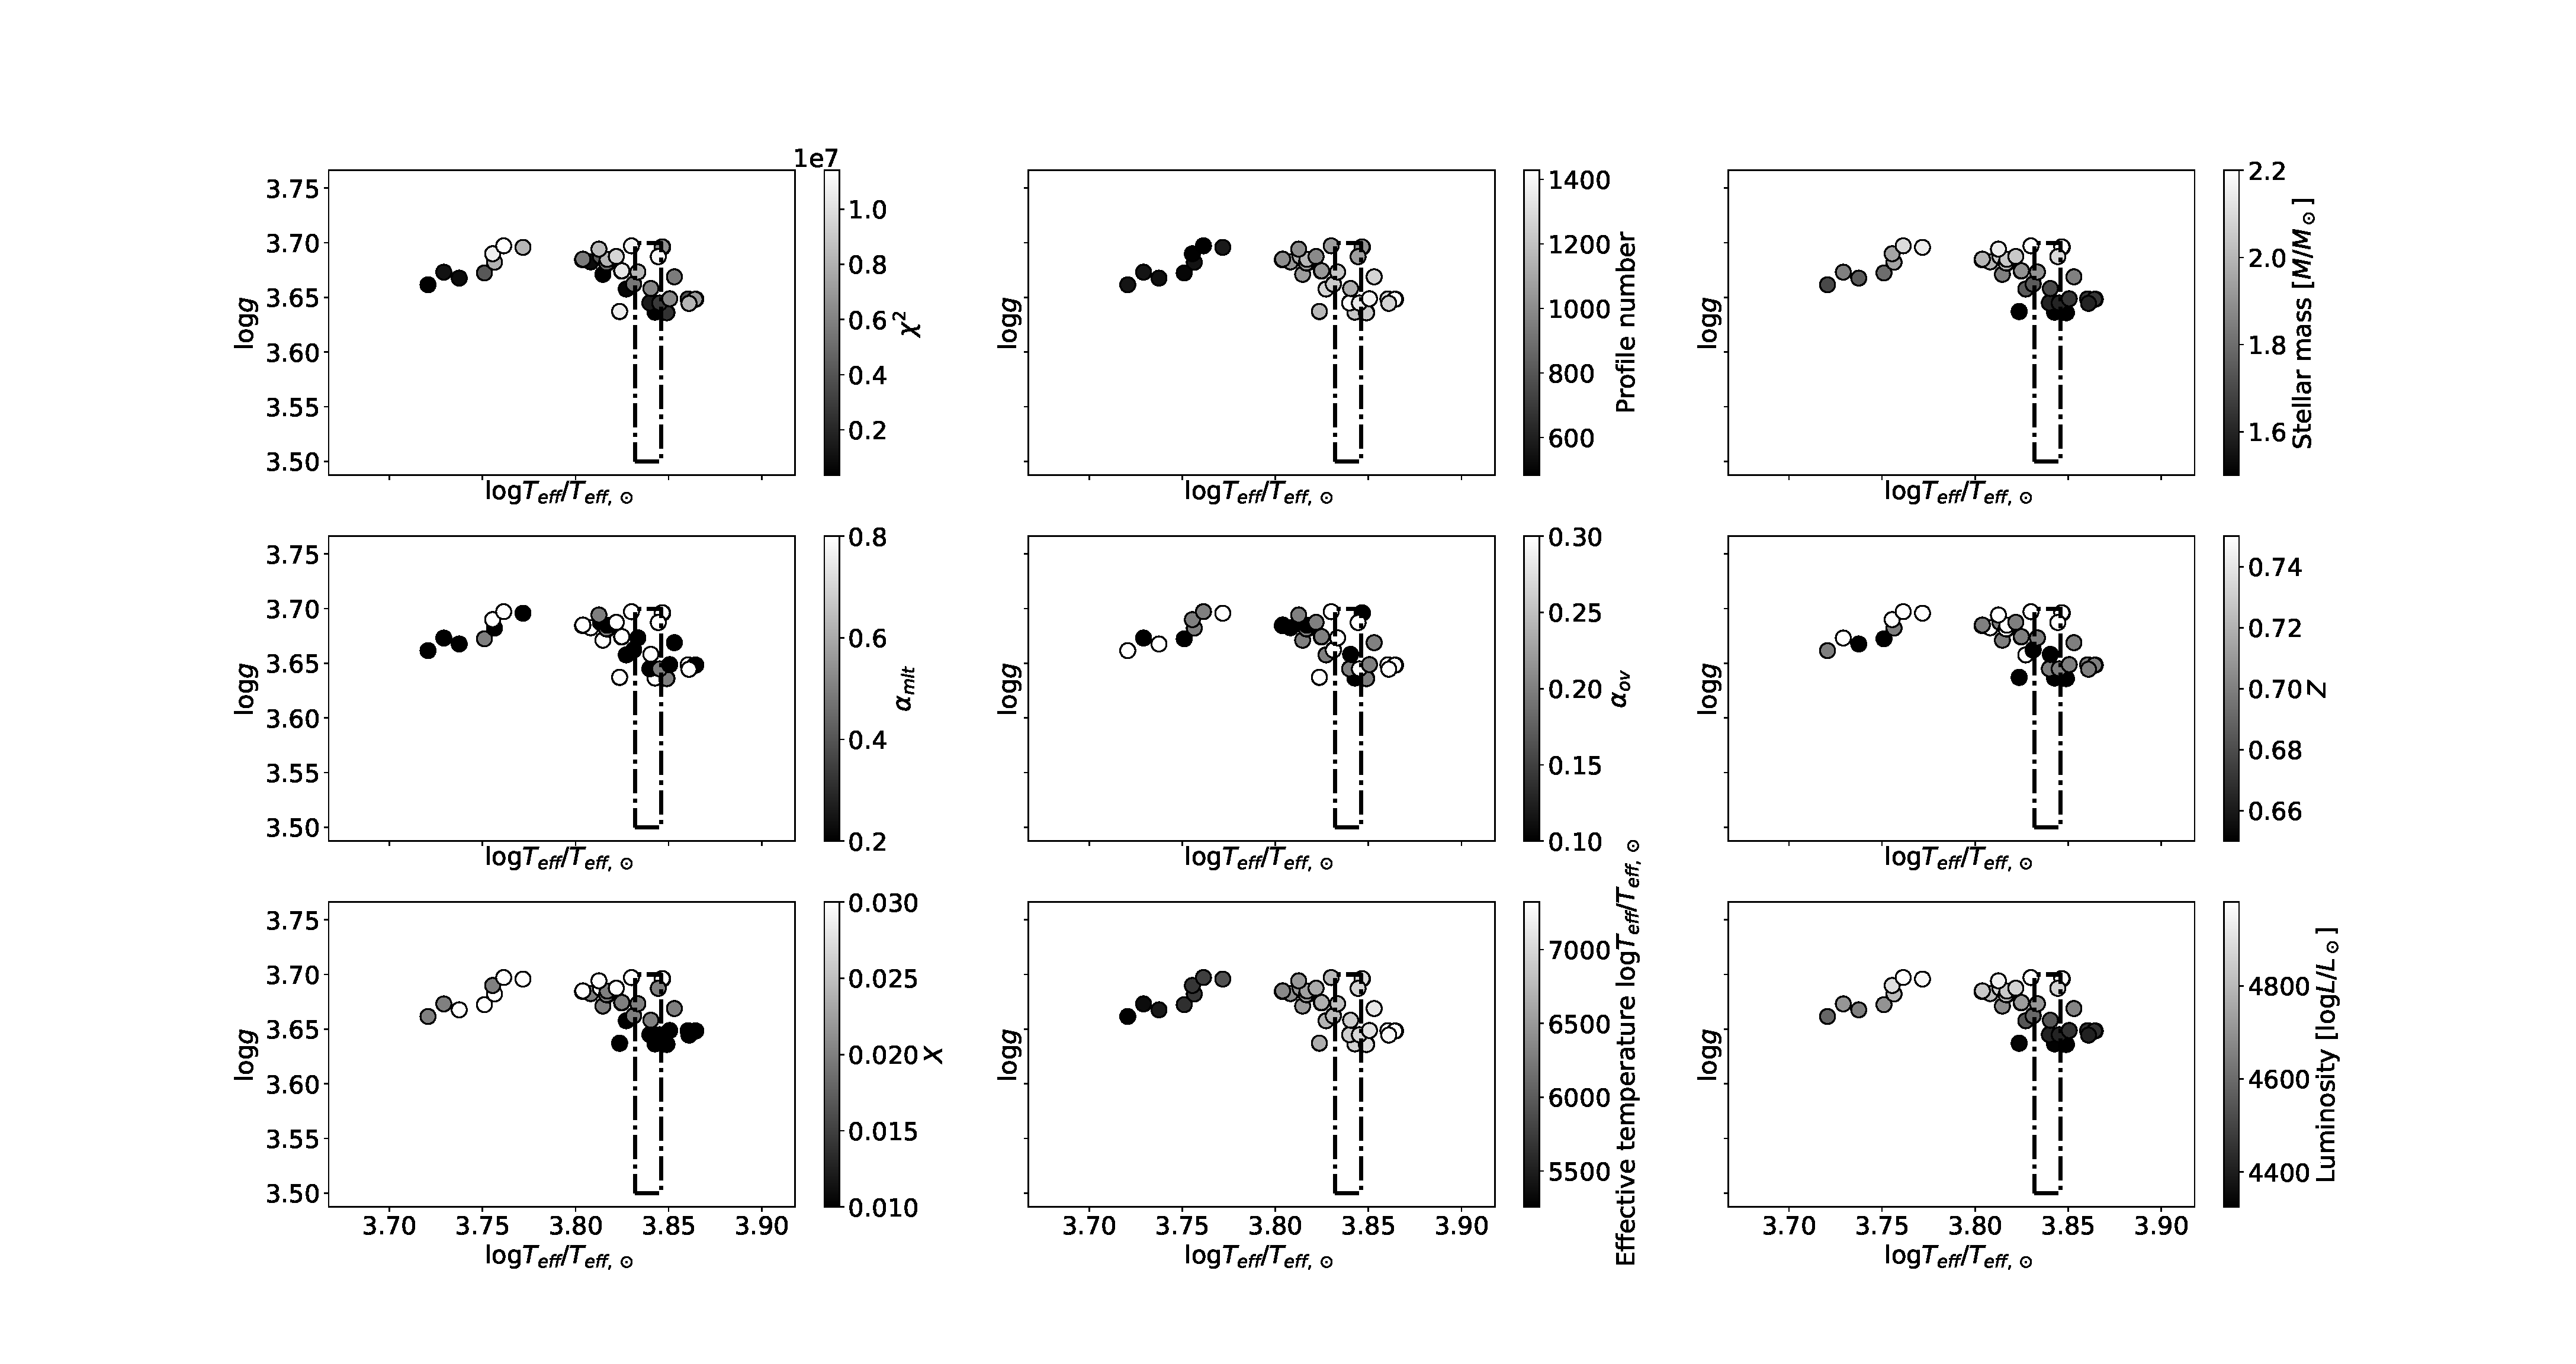
\includegraphics[width=1\textwidth]{scatter_all_v2.eps}
%	\makebox[\textwidth][c]{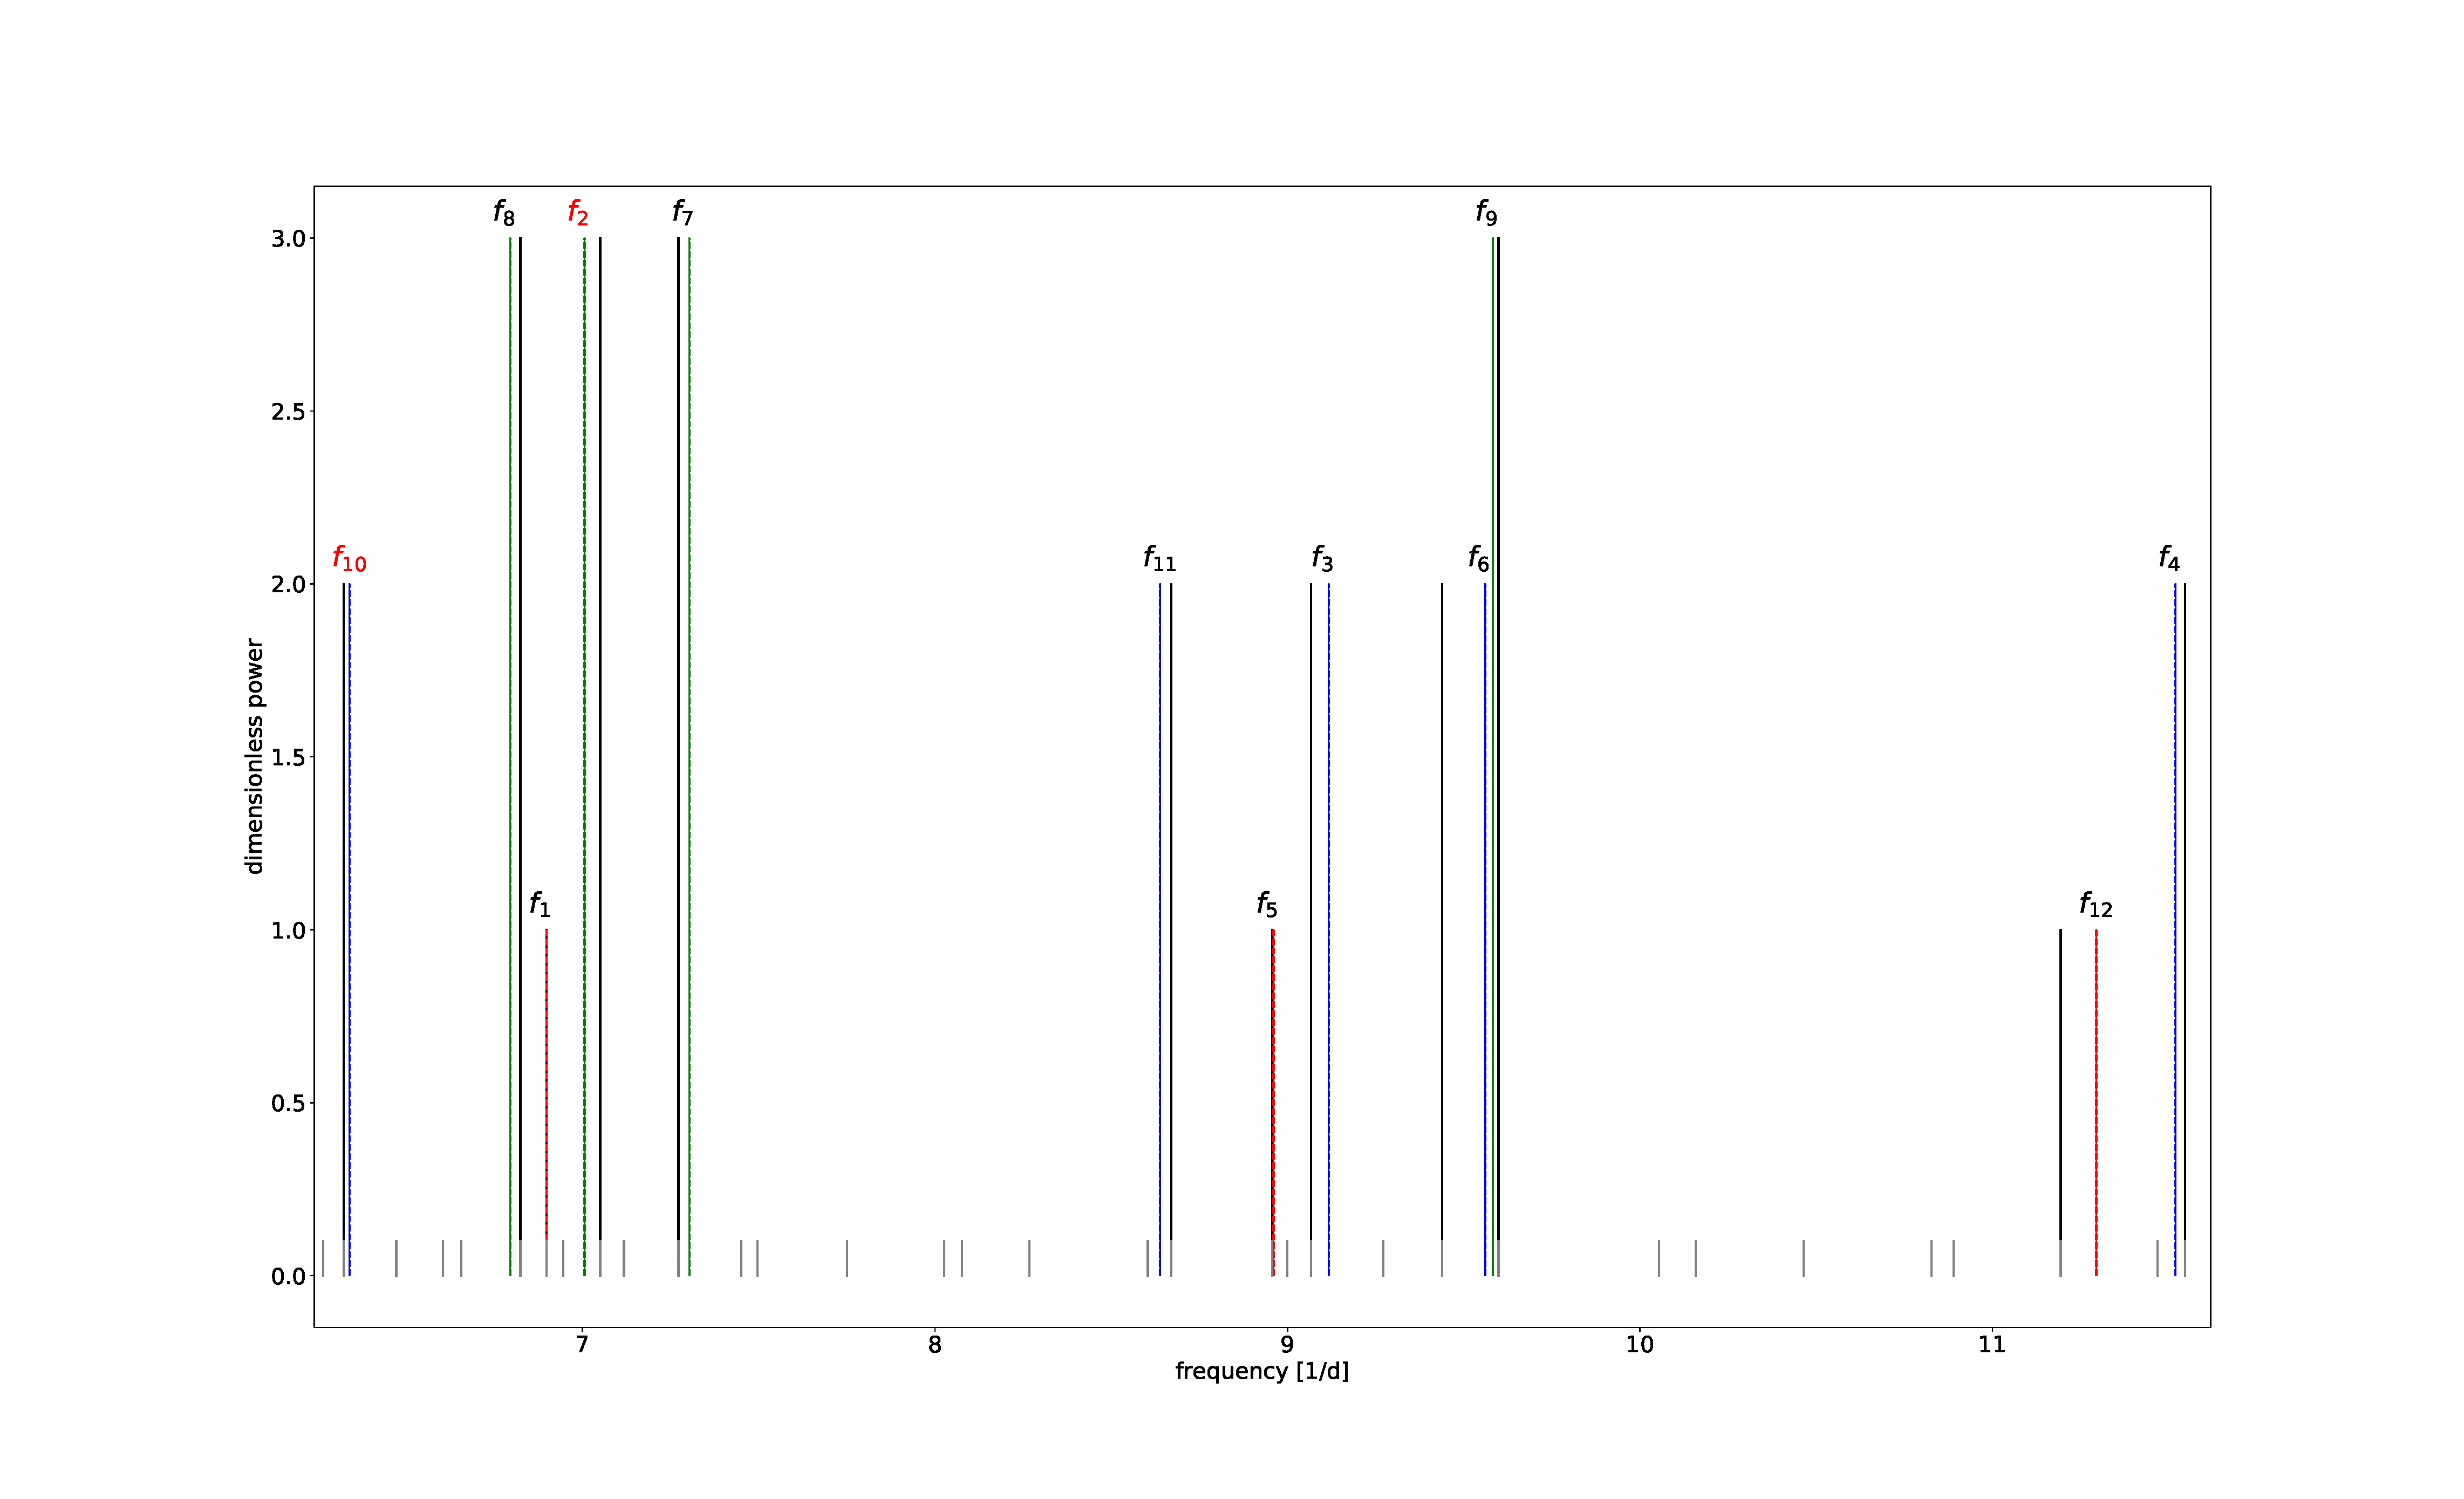
\includegraphics[width=1.5\textwidth]{frequency_fit.eps}}%
%	\caption{}
%	\label{}
%\end{figure}